%==============================================================================
% tento soubor pouzijte jako zaklad
% this file should be used as a base for the thesis
% Autoři / Authors: 2008 Michal Bidlo, 2018 Jaroslav Dytrych
% Kontakt pro dotazy a připomínky: dytrych@fit.vutbr.cz
% Contact for questions and comments: dytrych@fit.vutbr.cz
%==============================================================================
% kodovani: UTF-8 (zmena prikazem iconv, recode nebo cstocs)
% encoding: UTF-8 (you can change it by command iconv, recode or cstocs)
%------------------------------------------------------------------------------
% zpracování / processing: make, make pdf, make clean
%==============================================================================
% Soubory, které je nutné upravit: / Files which have to be edited:
%   xkocic01-Detekce-dopravnich-znacek-20-literatura-bibliography.bib - literatura / bibliography
%   xkocic01-Detekce-dopravnich-znacek-01-kapitoly-chapters.tex - obsah práce / the thesis content
%   xkocic01-Detekce-dopravnich-znacek-30-prilohy-appendices.tex - přílohy / appendices
%==============================================================================
%\documentclass[]{fitthesis} % bez zadání - pro začátek práce, aby nebyl problém s překladem
%\documentclass[english]{fitthesis} % without assignment - for the work start to avoid compilation problem
\documentclass[zadani]{fitthesis} % odevzdani do wisu a/nebo tisk s barevnými odkazy - odkazy jsou barevné
%\documentclass[english,zadani]{fitthesis} % for submission to the IS FIT and/or print with color links - links are color
%\documentclass[zadani,print]{fitthesis} % pro černobílý tisk - odkazy jsou černé
%\documentclass[english,zadani,print]{fitthesis} % for the black and white print - links are black
%\documentclass[zadani,cprint]{fitthesis} % pro barevný tisk - odkazy jsou černé, znak VUT barevný
%\documentclass[english,zadani,cprint]{fitthesis} % for the print - links are black, logo is color
% * Je-li práce psaná v anglickém jazyce, je zapotřebí u třídy použít 
%   parametr english následovně:
%   If thesis is written in english, it is necessary to use 
%   parameter english as follows:
%      \documentclass[english]{fitthesis}
% * Je-li práce psaná ve slovenském jazyce, je zapotřebí u třídy použít 
%   parametr slovak následovně:
%   If the work is written in the Slovak language, it is necessary 
%   to use parameter slovak as follows:
%      \documentclass[slovak]{fitthesis}
% * Je-li práce psaná v anglickém jazyce se slovenským abstraktem apod., 
%   je zapotřebí u třídy použít parametry english a enslovak následovně:
%   If the work is written in English with the Slovak abstract, etc., 
%   it is necessary to use parameters english and enslovak as follows:
%      \documentclass[english,enslovak]{fitthesis}

% Základní balíčky jsou dole v souboru šablony fitthesis.cls
% Basic packages are at the bottom of template file fitthesis.cls
% zde můžeme vložit vlastní balíčky / you can place own packages here

% Kompilace po částech (rychlejší, ale v náhledu nemusí být vše aktuální)
% Compilation piecewise (faster, but not all parts in preview will be up-to-date)
% \usepackage{subfiles}

% Nastavení cesty k obrázkům
% Setting of a path to the pictures
%\graphicspath{{obrazky-figures/}{./obrazky-figures/}}
%\graphicspath{{obrazky-figures/}{../obrazky-figures/}}

%---rm---------------
\renewcommand{\rmdefault}{lmr}%zavede Latin Modern Roman jako rm / set Latin Modern Roman as rm
%---sf---------------
\renewcommand{\sfdefault}{qhv}%zavede TeX Gyre Heros jako sf
%---tt------------
\renewcommand{\ttdefault}{lmtt}% zavede Latin Modern tt jako tt

% vypne funkci šablony, která automaticky nahrazuje uvozovky,
% aby nebyly prováděny nevhodné náhrady v popisech API apod.
% disables function of the template which replaces quotation marks
% to avoid unnecessary replacements in the API descriptions etc.
\csdoublequotesoff

% =======================================================================
% balíček "hyperref" vytváří klikací odkazy v pdf, pokud tedy použijeme pdflatex
% problém je, že balíček hyperref musí být uveden jako poslední, takže nemůže
% být v šabloně
% "hyperref" package create clickable links in pdf if you are using pdflatex.
% Problem is that this package have to be introduced as the last one so it 
% can not be placed in the template file.
\ifWis
\ifx\pdfoutput\undefined % nejedeme pod pdflatexem / we are not using pdflatex
\else
  \usepackage{color}
  \usepackage[unicode,colorlinks,hyperindex,plainpages=false,pdftex]{hyperref}
  \definecolor{hrcolor-ref}{RGB}{223,52,30}
  \definecolor{hrcolor-cite}{HTML}{2F8F00}
  \definecolor{hrcolor-urls}{HTML}{092EAB}
  \hypersetup{
  linkcolor=hrcolor-ref,
  citecolor=hrcolor-cite,
  filecolor=magenta,
  urlcolor=hrcolor-urls
  }
  \def\pdfBorderAttrs{/Border [0 0 0] }  % bez okrajů kolem odkazů / without margins around links
  \pdfcompresslevel=9
\fi
\else % pro tisk budou odkazy, na které se dá klikat, černé / for the print clickable links will be black
\ifx\pdfoutput\undefined % nejedeme pod pdflatexem / we are not using pdflatex
\else
  \usepackage{color}
  \usepackage[unicode,colorlinks,hyperindex,plainpages=false,pdftex,urlcolor=black,linkcolor=black,citecolor=black]{hyperref}
  \definecolor{links}{rgb}{0,0,0}
  \definecolor{anchors}{rgb}{0,0,0}
  \def\AnchorColor{anchors}
  \def\LinkColor{links}
  \def\pdfBorderAttrs{/Border [0 0 0] } % bez okrajů kolem odkazů / without margins around links
  \pdfcompresslevel=9
\fi
\fi
% Řešení problému, kdy klikací odkazy na obrázky vedou za obrázek
% This solves the problems with links which leads after the picture
\usepackage[all]{hypcap}

% Definice
\newtheorem{theorem}{Definice}

% Floating package
\usepackage{float}

% Reference na seznam
\usepackage{enumitem}

\usepackage{booktabs}
\usepackage{tabularx}
\usepackage{csquotes}
\usepackage{dsfont}
\usepackage{caption}

% Informace o práci/projektu / Information about the thesis
%---------------------------------------------------------------------------
\projectinfo{
  %Prace / Thesis
  project={BP},            %typ práce BP/SP/DP/DR  / thesis type (SP = term project)
  year={2019},             % rok odevzdání / year of submission
  date={15. 5. 2019},             % datum odevzdání / submission date
  %Nazev prace / thesis title
  title.cs={Detekce dopravních značek v obraze\\ a videu},  % název práce v češtině či slovenštině (dle zadání) / thesis title in czech language (according to assignment)
  title.en={Detection of Traffic Signs in Image and Video}, % název práce v angličtině / thesis title in english
  %title.length={14.5cm}, % nastavení délky bloku s titulkem pro úpravu zalomení řádku (lze definovat zde nebo níže) / setting the length of a block with a thesis title for adjusting a line break (can be defined here or below)
  %Autor / Author
  author.name={Filip},   % jméno autora / author name
  author.surname={Kočica},   % příjmení autora / author surname 
  %author.title.p={Bc.}, % titul před jménem (nepovinné) / title before the name (optional)
  %author.title.a={Ph.D.}, % titul za jménem (nepovinné) / title after the name (optional)
  %Ustav / Department
  department={UPGM}, % doplňte příslušnou zkratku dle ústavu na zadání: UPSY/UIFS/UITS/UPGM / fill in appropriate abbreviation of the department according to assignment: UPSY/UIFS/UITS/UPGM
  % Školitel / supervisor
  supervisor.name={Adam},   % jméno školitele / supervisor name 
  supervisor.surname={Herout},   % příjmení školitele / supervisor surname
  supervisor.title.p={prof. Ing.},   %titul před jménem (nepovinné) / title before the name (optional)
  supervisor.title.a={Ph.D.},    %titul za jménem (nepovinné) / title after the name (optional)
  % Klíčová slova / keywords
  keywords.cs={konvoluční neuronová síť, YOLO, detekce, klasifikace, syntetická, reálná, datová sada, dopravní značka}, % klíčová slova v českém či slovenském jazyce / keywords in czech or slovak language
  keywords.en={convolutional neural network, YOLO, detection, classification, synthetic, real, dataset, traffic sign}, % klíčová slova v anglickém jazyce / keywords in english
  %keywords.en={Here, individual keywords separated by commas will be written in English.},
  % Abstrakt / Abstract
  abstract.cs={Tato práce řeší problematiku detekce dopravního značení za pomoci moderních technik zpracování obrazu. K~řešení byla použita speciální architektura hluboké konvoluční neuronové sítě zvaná YOLO, tedy You Only Look Once, která řeší detekci i~klasifikaci objektů v~jednom kroce, což celý proces značně urychluje. Práce pojednává také o~porovnání úspěšnosti modelů trénovaných na reálných a~syntetických datových sadách. Podařilo se dosáhnout úspěšnosti $63.4\,\%$ mAP při použití modelu trénovaného na reálných datech a~úspěšnosti $82.3\,\%$ mAP při použití modelu trénovaného na datech syntetických. Vyhodnocení jednoho snímku trvá na průměrně výkonném grafickém čipu $\sim40.4\,\mathrm{ms}$ a~na nadprůměrně výkonném čipu $\sim3.9\,\mathrm{ms}$. Přínosem této práce je skutečnost, že model neuronové sítě trénovaný na syntetických datech může za určitých podmínek dosahovat podobných či lepších výsledků, než model trénovaný na reálných datech. To může usnadnit proces tvorby detektoru o~nutnost anotovat velké množství obrázků.},%Abstrakt
  abstract.en={This thesis deals with the traffic sign detection problematics using modern techniques in image processing. Special architecture of deep convolutional neural network YOLO, i.e. You Only Look Once, which performs both detection and classification in one step, has been used. This architecture allows object detector to work on very high speeds. This thesis also deals with comparison of models trained on real and synthetic datasets. The best model trained on real dataset has reached $63.4\,\%$ mAP success rate and $82.3\,\%$ mAP when trained on synthetic dataset. Evaluation of one image takes about $\sim40.4\,\mathrm{ms}$ on average graphics processing unit and $\sim3.9\,\mathrm{ms}$ on higher than average graphics processing unit. The benefit of this thesis is that under certain conditions neural network model trained on synthetic data can achieve same or even better results than model trained on real data. This may simplify process of object detector development since it is not necessary to annotate large number of images.},%Abstract
  % Prohlášení (u anglicky psané práce anglicky, u slovensky psané práce slovensky) / Declaration (for thesis in english should be in english)
  declaration={Prohlašuji, že jsem tuto bakalářskou práci vypracoval samostatně pod vedením pana prof. Ing. Adama Herouta, Ph.D. Uvedl jsem všechny literární prameny a publikace, ze kterých jsem čerpal.},
  %declaration={Hereby I declare that this bachelor's thesis was prepared as an original author’s work under the supervision of Mr. X
% The supplementary information was provided by Mr. Y
% All the relevant information sources, which were used during preparation of this thesis, are properly cited and included in the list of references.},
  % Poděkování (nepovinné, nejlépe v jazyce práce) / Acknowledgement (optional, ideally in the language of the thesis)
  acknowledgment={Zde bych rád poděkoval svému vedoucímu práce prof. Ing. Adamu Heroutovi, Ph.D za cenné rady, podnětné připomínky a vstřícnost při konzultacích. Dále děkuji za přístup k výpočetním a úložným zařízením ve vlastnictví stran a projektů, přispívajících k Národní Infrastruktuře Metacentrum v rámci programu \uv{Projects of Large Research, Development, and Innovations Infrastructures (CESNET LM2015042)}.},
  %acknowledgment={Here it is possible to express thanks to the supervisor and to the people which provided professional help
%(external submitter, consultant, etc.).},
  % Rozšířený abstrakt (cca 3 normostrany) - lze definovat zde nebo níže / Extended abstract (approximately 3 standard pages) - can be defined here or below
  %extendedabstract={Do tohoto odstavce bude zapsán rozšířený výtah (abstrakt) práce v českém (slovenském) jazyce.},
  %faculty={FIT}, % FIT/FEKT/FSI/FA/FCH/FP/FAST/FAVU/USI/DEF
  faculty.cs={Fakulta informačních technologií}, % Fakulta v češtině - pro využití této položky výše zvolte fakultu DEF / Faculty in Czech - for use of this entry select DEF above
  faculty.en={Faculty of Information Technology}, % Fakulta v angličtině - pro využití této položky výše zvolte fakultu DEF / Faculty in English - for use of this entry select DEF above
  department.cs={ÚSTAV POČÍTAČOVÉ GRAFIKY A MULTIMÉDIÍ}, % Ústav v češtině - pro využití této položky výše zvolte ústav DEF nebo jej zakomentujte / Department in Czech - for use of this entry select DEF above or comment it out
  department.en={DEPARTMENT OF COMPUTER GRAPHICS AND MULTIMEDIA} % Ústav v angličtině - pro využití této položky výše zvolte ústav DEF nebo jej zakomentujte / Department in English - for use of this entry select DEF above or comment it out
}

% Rozšířený abstrakt (cca 3 normostrany) - lze definovat zde nebo výše / Extended abstract (approximately 3 standard pages) - can be defined here or above
%\extendedabstract{Do tohoto odstavce bude zapsán výtah (abstrakt) práce v českém (slovenském) jazyce.}

% nastavení délky bloku s titulkem pro úpravu zalomení řádku - lze definovat zde nebo výše / setting the length of a block with a thesis title for adjusting a line break - can be defined here or above
%\titlelength{14.5cm}


% řeší první/poslední řádek odstavce na předchozí/následující stránce
% solves first/last row of the paragraph on the previous/next page
\clubpenalty=10000
\widowpenalty=10000

% checklist
\newlist{checklist}{itemize}{1}
\setlist[checklist]{label=$\square$}

\begin{document}
  % Vysazeni titulnich stran / Typesetting of the title pages
  % ----------------------------------------------
  \maketitle
  % Obsah
  % ----------------------------------------------
  \setlength{\parskip}{0pt}

  {\hypersetup{hidelinks}\tableofcontents}
  
  % Seznam obrazku a tabulek (pokud prace obsahuje velke mnozstvi obrazku, tak se to hodi)
  % List of figures and list of tables (if the thesis contains a lot of pictures, it is good)
  \ifczech
    \renewcommand\listfigurename{Seznam obrázků}
  \fi
  \ifslovak
    \renewcommand\listfigurename{Zoznam obrázkov}
  \fi
  % \listoffigures
  
  \ifczech
    \renewcommand\listtablename{Seznam tabulek}
  \fi
  \ifslovak
    \renewcommand\listtablename{Zoznam tabuliek}
  \fi
  % \listoftables 

  \ifODSAZ
    \setlength{\parskip}{0.5\bigskipamount}
  \else
    \setlength{\parskip}{0pt}
  \fi

  % vynechani stranky v oboustrannem rezimu
  % Skip the page in the two-sided mode
  \iftwoside
    \cleardoublepage
  \fi

  % Text prace / Thesis text
  % ----------------------------------------------
  \chapter{Úvod}
Asistenční systémy pro řidiče a~autonomní vozidla se v~posledních letech dočkaly velké pozornosti. Stojí zejména na správné interpretaci okolního prostředí, kam mj. spadá problematika detekce dopravního značení. Ta má stále prostor pro zlepšení. S~nárůstem výpočetního výkonu velmi vzrostlo použití hlubokých neuronových sítí pro různé úlohy, zejména pak pro zpracování obrazu, kde se konvoluční sítě staly standardem pro velkou část úloh. Proto je vhodné pokusit se řešit problém detekce značek pomocí této metody.

%--------------------------------------------------------

Nevýhodou drtivé většiny metod používajících konvoluční sítě k~detekci objektů a~zároveň dosahujících dobrých výsledků jsou vysoké nároky na výpočetní výkon (což znesnadňuje jejich použití v~přenosných či vestavěných zařízeních) a~dlouhá doba zpracování jednoho snímku -- oba zmíněné systémy však musí dokázat pracovat v~reálném čase v~kombinaci s~velmi dobrou úspěšností detekce.
I~když se detekce značek může zdát jako jednoduchá, existuje velké množství faktorů, které tuto úlohu znesnadňují (různé světelné podmínky, částečné překrytí, malá velikost, nízká kvalita, atd.). Proto je potřeba dostatečně velká datová sada, obsahující co největší množství i~těchto negativních faktorů. Proces anotace velkého počtu snímků je ovšem velmi náročný na čas (mj. může vzniknout chybná anotace).
Ideálním řešením by tedy byl úspěšný systém, který by dokázal pracovat v~reálném čase na zařízení s~omezeným výpočetním výkonem a~byl by schopen se naučit dostatek informací i~ze syntetických dat.

%--------------------------------------------------------

Za účelem dosažení zpracování v~reálném čase na běžně dostupných grafických čipech se zachováním dobré úspěšnosti byl pro práci vybrán systém Tiny YOLO třetí verze v~kombinaci s~neuronovou sítí Darknet.
Generování datových sad pro trénování neuronových sítí je aktuálně velmi diskutovaným tématem a~lze využít více způsobů v~závislosti na typu generovaných dat. Z~důvodu, že je systém YOLO trénovaný na plných snímcích a~dopravní značky nabývají poměrně jednoduchých tvarů, byl využit způsob umisťování dopravních značek do plných snímků z~prostředí městské zástavby.

%--------------------------------------------------------

Cílem tohoto dokumentu je jednak podat čtenáři krátký přehled o~možnostech řešení problematiky detekce dopravního značení, dále pak popsat způsob řešení dané problematiky v~rámci této práce a~nakonec vyhodnotit dosažené výsledky.
Struktura dokumentu je tedy následující.
Kapitola \ref{detekceZnacek} se zabývá popisem dopravního značení, metod detekce značek používaných v~minulosti, metrik používaných k~vyhodnocení úspěšnosti detekce objektů a~nakonec porovnáním existujících řešení.
Kapitola \ref{detekceKonv} je zaměřena na popis moderních technik detekce objektů založených na konvolučních neuronových sítích.
V~kapitole \ref{navrhDetektoru} je popsán návrh řešení, což zahrnuje výběr metody, datových sad a~návrh generátoru syntetických dat.
Implementací a~testováním zvolené metody se zabývá kapitola \ref{implementaceDetektoru} a~nakonec dosažené výsledky a~jejich zhodnocení lze najít v~kapitole \ref{vyhodnoceniDetektoru}.


\chapter{Detekce dopravního značení}
\label{detekceZnacek}
Tato kapitola pojednává o~obecném popisu dopravního značení, jehož automatizované rozpoznání pomocí počítače je cílem této práce. Dále jsou v~této kapitole popsány běžně používané metody pro detekci a~klasifikaci dopravního značení v~současné době, a~také metriky používané pro vyhodnocení úspěšnosti v~oboru detekce objektů. Nakonec jsou zmíněny zajímavé existující práce z~této oblasti, jimi použité metody a~dosažené výsledky.


%%%%%%%%%%%%%%%%%%%%%%%%%%%%%%%%%%%%%%%%%%%%%%%%%%%%%%%%%%%%%%%%%%%%%%%%%%%%%%%%%%%%%%%%%%%


\section{Dopravní značení}
\label{dopravniZnaceni}
Dopravní značení slouží k~účelu řízení a~regulace dopravy na pozemních komunikacích a~tedy k~zajištění plynulosti a~bezpečnosti dopravy. Svislé dopravní značení, kterému se tato práce věnuje, se běžně nachází na stranách silnice či na konstrukci nad silnicí \cite{dopravniZnacka, dopravniZnaceniVCesku}.

\subsection*{Dělení dopravního značení v~Česku}
\label{dopravniZnaceniDeleni}
Dělení svislého dopravního značení, které je nejčastějším způsobem dopravního značení, se skládá ze šesti tříd vizualizovaných na obrázku \ref{kolazDopravniZnacky} a~jejich krátký popis podle \cite{seznamDopravnichZnacek, dopravniZnacka, dopravniZnaceniVCesku} je následovný:

\begin{itemize}
    \item \textbf{Výstražné dopravní značky} upozorňují účastníky silničního provozu na možná nebezpečí a~rizika. Jsou to zpravidla trojúhelníky s~bílým pozadím, piktogramem uprostřed a~ohraničené červenou barvou.
    \item \textbf{Značky upravující přednost} se používají na křižovatkách pro určení přednosti. Tyto značky mohou být trojúhelníkové, čtvercové i~osmiúhelníkové a~barevné provedení je buďto žluté, červené či modré.
    \item \textbf{Zákazové dopravní značky} ukládají účastníkům silničního provozu zákazy jistých činností.
    \item \textbf{Příkazové dopravní značky} slouží k~odstranění možnosti vzniku nebezpečných situací. Tyto značky jsou vždy kruhového tvaru s~modrým barevným provedením a~bílým piktogramem či textem uprostřed.
    \item \textbf{Informativní dopravní značky} poskytují pro účastníky silničního provozu důležité informace, určující například orientaci, typ zóny či silnice.
    \item \textbf{Dodatkové tabulky} slouží k~doplnění či omezení významu jiných dopravních značek. 
\end{itemize}

\begin{figure}[H]
    \centering
    \tmpframe{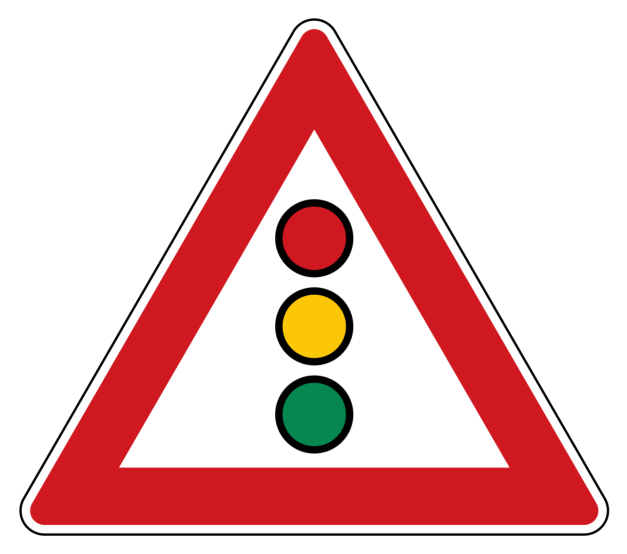
\includegraphics[width=0.15\linewidth]{figures/znacky/vystrazne.eps}}
    \tmpframe{
\includegraphics[width=0.15\linewidth]{figures/znacky/prednost}}
    \tmpframe{
\includegraphics[width=0.15\linewidth]{figures/znacky/zakazove}}
    \tmpframe{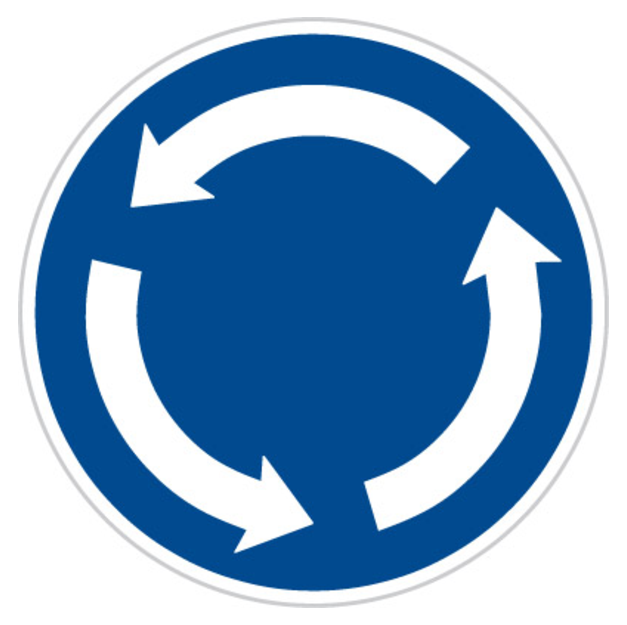
\includegraphics[width=0.15\linewidth]{figures/znacky/prikazove}}
    \tmpframe{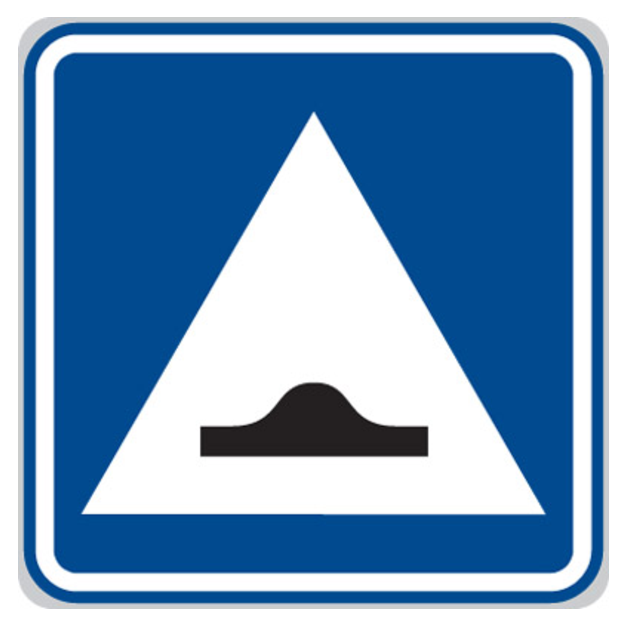
\includegraphics[width=0.15\linewidth]{figures/znacky/informativni}}
    \tmpframe{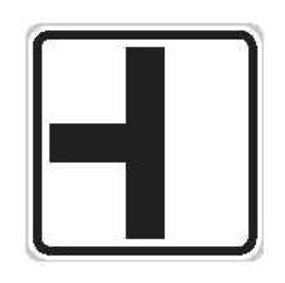
\includegraphics[width=0.15\linewidth]{figures/znacky/dodatkove}}
    \caption{Příklad značek jednotlivých tříd.\footnotemark}
    \label{kolazDopravniZnacky}
\end{figure}

\footnotetext{Převzato z~\cite{seznamDopravnichZnacek}.}

\subsection*{Vzhled dopravních značek}
\label{dopravniZnaceniBarvy}
Evropská norma definuje základní vlastnosti značek, ale ponechává státům jistou volnost. Značky v~jednotlivých státech se mohou trochu lišit, ať už barvou, velikostí či tvarem. Pro člověka je tento rozdíl téměř nevnímatelný, ale počítači může při detekci působit potíže. Na obrázku \ref{kolazStopky} lze vidět variabilitu barev a~způsobu zpracování značek \emph{stop} pěti Evropských států (Rakouska, Česka, Řecka, Rumunska a~Turecka) \cite{dopravniZnacka}.

\begin{figure}[H]
    \centering
    \tmpframe{
\includegraphics[width=0.19\linewidth]{figures/znacky/rakouske}}\hfill
    \tmpframe{
\includegraphics[width=0.19\linewidth]{figures/znacky/ceske}}\hfill
    \tmpframe{
\includegraphics[width=0.19\linewidth]{figures/znacky/recke}}\hfill
    \tmpframe{
\includegraphics[width=0.19\linewidth]{figures/znacky/rumunske}}\hfill
    \tmpframe{
\includegraphics[width=0.19\linewidth]{figures/znacky/turecke}}
    \caption{Rozdílnost značek stop některých Evropských zemí.\footnotemark}
    \label{kolazStopky}
\end{figure}

\footnotetext{Převzato z~\url{https://en.wikipedia.org/wiki/Comparison_of_European_road_signs}}

Ačkoli se detekce dopravních značek může zdát jako jednoduchá úloha, tak stále není úplně vyřešena a~stále přibývají kvalitní práce posouvající tuto problematiku kupředu. Velký problém při detekci značek sehrávají různé světelné podmínky, přírodní vlivy (např. vyblednutí barev, sníh, déšť), vandalismus, deformace či jiné poškození značek, částečné překrytí, malá velikost, apod., jak lze vidět na obrázku \ref{fig:kolazZnacky}.

\begin{figure}[H]
    \centering
    \tmpframe{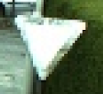
\includegraphics[width=0.20\linewidth]{figures/detekce/bad_conditions/bad_sign_1.png}}\hfill
    \tmpframe{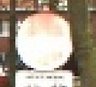
\includegraphics[width=0.20\linewidth]{figures/detekce/bad_conditions/bad_sign_2.png}}\hfill
    \tmpframe{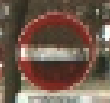
\includegraphics[width=0.20\linewidth]{figures/detekce/bad_conditions/bad_sign_3.png}}\hfill
    \tmpframe{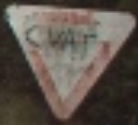
\includegraphics[width=0.20\linewidth]{figures/detekce/bad_conditions/bad_sign_4.png}}\\
    \tmpframe{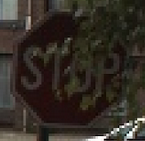
\includegraphics[width=0.20\linewidth]{figures/detekce/bad_conditions/bad_sign_5.png}}\hfill
    \tmpframe{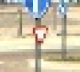
\includegraphics[width=0.20\linewidth]{figures/detekce/bad_conditions/bad_sign_6.png}}\hfill
    \tmpframe{
\includegraphics[width=0.20\linewidth]{figures/detekce/bad_conditions/bad_sign_7.png}}\hfill
    \tmpframe{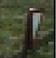
\includegraphics[width=0.20\linewidth]{figures/detekce/bad_conditions/bad_sign_8.png}}
    \caption{Problémové dopravní značky pocházející z použité datové sady.}
    \label{fig:kolazZnacky}
\end{figure}

%%%%%%%%%%%%%%%%%%%%%%%%%%%%%%%%%%%%%%%%%%%%%%%%%%%%%%%%%%%%%%%%%%%%%%%%%%%%%%%%%%%%%%%%%%%

\section{Způsoby detekce dopravního značení}
\label{zpusobyDetekce}
Při detekci těchto objektů lze vycházet z~jejich specifického tvaru, barvy a~také jejich dobré rozlišitelnosti od pozadí \cite{tsDetectOverview}. Vzhledem k~množství již existujících prací na toto téma se nabízí celá řada způsobů, jak k~řešení tohoto problému přistupovat, proto zde bude zmíněno jen několik nejdůležitějších. Problém lze řešit také pomocí konvolučních neuronových sítí, popsaných samostatně v~kapitole \ref{detekceKonv}. Na rozdíl od klasifikace objektů, jejich detekce vyžaduje lokalizaci (běžně více) objektů v~rámci celého snímku \cite{rcnn}.

\subsection*{Segmentace na základě barvy}
\label{zpusobyDetekceSegmentace}
Základní segmentace obrazu je běžně dosažena pomocí prahování na základě určité barvy. Podle práce \cite{tsDetect} je intuitivní použití barevného modelu RGB (red, green, blue), u~kterého je každý pixel definován pomocí třech hodnot: červené, zelené a~modré. Prahování pomocí tohoto barevného modelu lze vyjádřit pomocí rovnic \eqref{eq:soustavaRGB1} a~\eqref{eq:soustavaRGB2}.
\begin{align}
    \label{eq:soustavaRGB1}
    g(x,y) &= k_1\begin{cases}
    \ R_a \leq f_r(x,y) \leq R_b\\
    \ G_a \leq f_g(x,y) \leq G_b\\
    \ B_a \leq f_b(x,y) \leq B_b\end{cases}\\
    \label{eq:soustavaRGB2}
    g(x,y) &= k_2 \text{ v~jakémkoli jiném případě}
\end{align}
Funkce $f_*(x,y)$ udávají hodnotu jednotlivých barevných složek daného bodu obrázku. Výsledný pixel nabývá hodnoty $k_1$ pouze v~případě, že všechny barevné kanály pixelu spadají do předem definovaných intervalů, jinak nabývá hodnoty $k_2$. Velkou nevýhodou tohoto barevného modelu ovšem je, že je velmi citlivý na změnu osvětlení. Z~tohoto důvodu se již v~75. letech minulého století zavedly nové barevné modely HS* (HSI, HSV, HSL), které jsou mnohem bližší lidskému vnímání barev \cite{tsDetectOverview}. První složka je \emph{hue}, tedy odstín. Druhá je \emph{saturation}, která udává sytost a~poslední např. \emph{intensity} (I), udávající intenzitu barvy. Převod z~barevného prostoru RGB, pomocí něhož jsou obrázky běžně reprezentovány, do jednoho ze zmíněných modelů byl v~minulosti výpočetně dosti náročný, ale s~dnešní výpočetní kapacitou to není problém, a~proto se často využívá. Převod z~barevného prostoru RGB do HSV podle \cite{tsRychlaDetekce} je následující:
\begin{align}
    \label{eq:soustavaHSV}
    V~&= max(R,G,B)\\
    S~&= \begin{cases}
    \ \frac{V~- min(R,G,B)}{V}  & V~\neq 0\\
    \ 0 & V~= 0\end{cases}\\
    H &= \begin{cases}
    \ \frac{60(G-B)}{V - min(R,G,B)} & V~= R \vspace{4px}\\
    \ \frac{120+60(B-R)}{V - min(R,G,B)} & V~= G\vspace{4px}\\
    \ \frac{240+60(R-G)}{V - min(R,G,B)} & V~= B\end{cases}
\end{align}
Z~tabulky porovnání detekčních metod v~\cite{tsDetectOverview} vyplývá, že je používaný jak barevný model RGB, použit $5\times$, tak barevný model HS*, použit také $5\times$. Mimo ně byl v~porovnání jedenkrát uveden model CIECAM97. Příklad použití prahování na základě červené barvy při použití modelu RGB lze vidět na obrázku~\ref{fig:prahovani}.

\begin{figure}[H]
    \centering
    \tmpframe{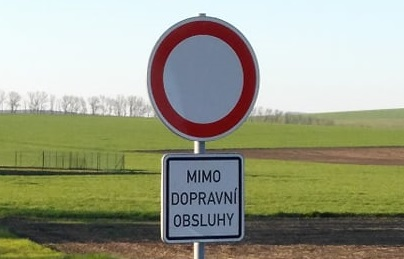
\includegraphics[width=0.495\linewidth]{figures/detekce/TS.png}}\hfill
    \tmpframe{
\includegraphics[width=0.495\linewidth]{figures/detekce/TS_thresholding.png}}
    \caption{Prahování na základě červené barvy pomocí barevného modelu RGB. Upraveno pomocí \texttt{OpenCV}.}
    \label{fig:prahovani}
\end{figure}


\subsection*{Cannyho hranový detektor}
\label{zpusobyDetekceCanny}
Tento detektor byl vytvořen v~roce 1986 Johnem Cannym, ale ještě dnes se v~oblasti zpracování obrazu hojně využívá \cite{canny}. Canny definoval základní pravidla, která musí detektor splňovat, a~ty jsou následovné:

\begin{enumerate}
    \item \textbf{Vysoká úroveň detekce}. Detektor by měl mít nízkou pravděpodobnost selhání detekce existující hrany a~zároveň nízkou pravděpodobnost detekce neexistující hrany.
    \item \textbf{Dobrá lokalizace}. Body označené jako hraniční by měly být co nejblíže středu reálné hrany.
    \item \textbf{Pouze jedna detekce jedné hrany}. Pokud je jedna hrana detekována vícekrát, pouze jedna z~těchto detekcí by měla být označena jako správná a~ostatní ignorovány.
\end{enumerate}

\begin{figure}[H]
    \centering
    \tmpframe{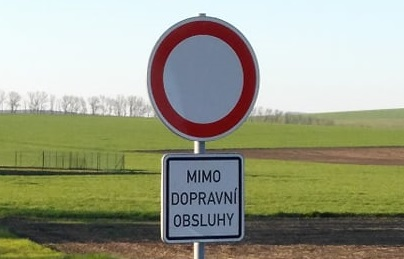
\includegraphics[width=0.495\linewidth]{figures/detekce/TS.png}}\hfill
    \tmpframe{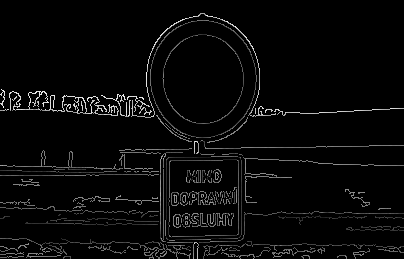
\includegraphics[width=0.495\linewidth]{figures/detekce/TS_canny.png}}
    \caption{Detekce hran pomocí Cannyho hranového detektoru. Upraveno pomocí \texttt{OpenCV}.}
    \label{fig:canny}
\end{figure}


Algoritmus je koncipován pouze pro práci se signálem obsahující jeden kanál, proto nelze metodu přímo použít například na RGB obrázek, který má tři kanály. První je potřeba převést obrázek do stupňů šedi. Výsledek detekce hran dopravní značky pomocí Cannyho detektoru lze vidět na obrázku \ref{fig:canny}. Obecný popis zpracování obrazového signálu Cannyho detektorem je následovný \cite{canny, tsRychlaDetekce, tsWindowsPhone}.

\begin{enumerate}
    \item Redukce šumu  -- provedení konvoluce obrazu $f$ s~gaussovým filtrem $G$, tedy $f * G$.
    \item Nalezení velikosti a~směru gradientu. $n$ by měla být orientovaná normála ke směru detekované hrany a~i~přesto, že tento směr není znám, je možné udělat jeho poměrně přesný odhad na základě směru vyhlazeného gradientu:
    \begin{align}
        \label{eq:soustavaCanny}
        n &= \frac{\nabla(G * f)}{|\nabla(G * f)|}
    \end{align}
    \item Nalezení správné pozice hrany pomocí operace zvané \emph{nonmaximum suppression}, tedy potlačení ne-maximálních hodnot. Ta slouží k~odstranění hodnot, které nejsou ve směru gradientu lokální maxima.
    \item Provést v~obraze prahování s~hysterezí pro odstranění bezvýznamných hran. Existují dva zadané prahy $T_1$ (minimální) a~$T_2$ (maximální). Pokud je odezva v~bodě vyšší než $T_2$, je bod označen za součást hrany. Pokud se odezva bodu nachází mezi $T_1$ a~$T_2$ a~zároveň je spojena s~bodem, který již byl označen jako součást hrany, je tento bod také označen za součást hrany. Všechny ostatní body jsou označeny tak, že nejsou považovány za součást žádné hrany.
\end{enumerate}

Velkou výhodou Cannyho detektoru hran je, že není citlivý na šum a~dokáže tedy pracovat se značně zašuměným obrazem \cite{tsDetekceTapuska}.


\subsection*{Detekce geometrických tvarů v~obraze pomocí Houghovy transformace}
\label{zpusobyDetekceHough}
Houghova transformace je výpočetně poměrně náročná operace, a~proto se na obraz běžně první aplikuje hranový detektor a~až poté se provádí Houghova transformace. Detekce hran vede k~poměrně značné redukci informace a~šumu v~obrazu a~zachová informaci potřebnou pro nalezení objektu. Proto podstatně zrychluje celý proces a~zpřesňuje výsledek. Pomocí Houghovy transformace se hledají tzv. ROI (\emph{Regions of Interest}, tedy oblasti zájmu), ve kterých se může dopravní značka nacházet. Metoda byla nesčetněkrát modifikována a~rozšířena~\cite{houghTransformace, tsDetekceSvoboda}.

\subsubsection{Klasická Houghova transformace}
\label{zpusobyDetekceHoughtKlasicka}
Houghova transformace pro detekci přímek vychází z~rovnice přímky \eqref{eq:rovnicePrimky}. Podle \cite{houghTransformace, tsWindowsPhone} libovolná přímka může být reprezentována pomocí jediného bodu v~prostoru. Parametr $\theta$ udává úhel, který svírá normála přímky s~kladnou částí osy $x$. Parametr $\rho$ udává vzdálenost přímky od středu souřadného systému.
\begin{align}
    \label{eq:rovnicePrimky}
    x \cos{\theta} + y \sin{\theta} = \rho
\end{align}
Tyto parametry je pro detekci přímky potřeba nalézt a~vytváří se pro tyto účely dvou-dimenzionální Houghův prostor složený z~parametrů $\theta$ a~$\rho$. Postupně se prochází celý prohledávaný prostor a~pro každý bod se určí všechny možné přímky procházející tímto bodem a~umístí se do zmíněného Houghova prostoru. Pro daný bod tedy vznikne sinusoida, viz obrázek \ref{fig:hough}. Sinusoidy všech bodů, které leží na stejné přímce, se protnou ve stejném bodě.

\begin{figure}[H]
    \centering
    \tmpframe{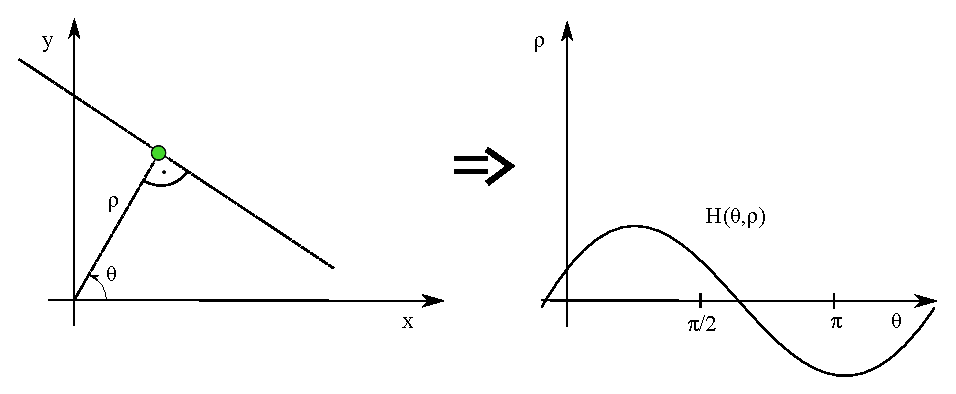
\includegraphics[width=0.9\linewidth]{figures/detekce/hough.eps}}
    \caption{Bod obrázku převedený na sinusoidu v~Houghově prostoru.}
    \label{fig:hough}
\end{figure}

\subsubsection{Zobecněná Houghova transformace}
\label{zpusobyDetekceHoughtZobecnena}
Stejně jako metoda pro detekci přímek vycházela z~rovnice přímky \eqref{eq:rovnicePrimky}, vychází metoda pro detekci kružnic z~rovnice kružnice \eqref{eq:rovniceKruznice}, kde $a$ a~$b$ udávají střed kružnice a~parametr $c$ udává poloměr kružnice.
\begin{align}
    \label{eq:rovniceKruznice}
    (x - a)^2 + (y - b)^2 = c
\end{align}
Postupuje se stejně jako u~detekce přímek, pouze jsou zde hledány tři parametry, a~proto Houghův prostor bude mít v~tomto případě tři dimenze.

\subsection*{Histogram orientovaných gradientů}
Při studiu této problematiky jsem vycházel z~práce \cite{hog}. Základní myšlenka je taková, že vzhled a~tvar objektu může být reprezentován pomocí intenzity gradientů bez nutnosti znát jeho přesnou polohu. Metoda funguje na principu rozdělení vstupního obrázku na menší části pevně dané velikosti zvané \emph{buňky} a~získávání normalizovaných lokálních histogramů gradientů těchto buněk. Každá buňka produkuje jednorozměrný histogram směru gradientů či orientace hran na základě pixelů nacházejících se v~buňce (každý pixel produkuje \emph{hlas}, které jsou akumulovány do lokálních kontejnerů -- zvýšení počtu těchto kontejnerů značně zlepšuje úspěšnost). Velikost gradientu závisí na lokálních změnách osvětlení, a~proto pro lepší odolnost vůči změně osvětlení je dobré provést normalizaci kontrastu.

Normalizace kontrastu lze dosáhnout pomocí získání celkového množství \uv{energie} histogramu na větším prostoru zvaném \emph{blok} a~pomocí výsledku normalizovat veškeré buňky, které se v~daném bloku nachází. Normalizace kontrastu se ukázala jako klíčová pro dosažení dobré úspěšnosti. Vektor těchto histogramů získaných z~jednoho bloku je nazývaný deskriptor. V~případě barevných obrázků jsou počítány gradienty pro každý kanál odděleně a~výsledným vektorem gradientu daného bodu se stává ten s~nejvyšší normalizovanou hodnotou.


%%%%%%%%%%%%%%%%%%%%%%%%%%%%%%%%%%%%%%%%%%%%%%%%%%%%%%%%%%%%%%%%%%%%%%%%%%%%%%%%%%%%%%%%%%%


\section{Způsoby klasifikace dopravního značení}
\label{zpusobyKlasifikace}
Po nalezení kandidátních oblastí (tzv. \emph{Regions of Interest}), ve kterých se mohou nacházet dopravní značky, je třeba rozhodnout, zda se v~tomto místě značka opravdu nachází, a~také značku klasifikovat do správné třídy. K~tomu lze využít následující metody.

\subsection*{Support Vector Machines -- SVM}
\label{SVM}
\emph{Support Vector Machines} (dále jen zkratka SVM) vytváří jednu či více hyper-rovin ve vícerozměrném prostoru použitých pro klasifikaci. Při studiu této metody jsem vycházel ze \cite{CVmodernApproach, classificMethodsComp3, tsDetekceSvoboda}. SVM je v~základní verzi binární klasifikátor, který dokáže klasifikovat data pouze dvou tříd, ale je možné jej použít také k~regresi a a-třídní klasifikaci. Trénovací data se skládají z~konečné sady $N$ bodů $x_i$, kde každý spadá do jedné ze dvou tříd, které jsou reprezentovány pomocí $y_i$ a~nabývají hodnot $1$ nebo $-1$. Taková datová sada potom může vypadat následovně:
\begin{align}
    \label{eq:svm0}
    x = \{(x_1,y_1),...,(x_N,y_N)\}
\end{align}
Pro lineárně odlišitelnou datovou sadu existují parametry $w$ a~$b$ (kde $w$ je vektor vah a~$b$ je práh reprezentující hyperrovinu) pro každý vstupní bod:
\begin{align}
    \label{eq:svm1}
    y_i(w \cdot x_i + b) > 0
\end{align}
Takovýto výraz existuje pro každý z~bodů vstupní datové sady a~tato sada výrazů poté definuje omezení na volbu parametrů $w$ a~$b$. Tato omezení vyjadřují, že všechny vstupní prvky se záporným $y_i$ by měly být na jedné straně hyper-roviny, zatímco prvky s~kladným $y_i$ na straně druhé. Při změně měřítek obou parametrů $w$ a~$b$ nedochází k~porušení podmínky vyjádřené pomocí \eqref{eq:svm1}, ale je možné zvolit parametry tak, aby platilo:
\begin{align}
    \label{eq:svm2}
    y_i(w \cdot x_i + b) \geq 1
\end{align}
Nejběžnější přístup k~vytvoření dělící hyper-roviny je takový, aby byla co nejdále od konvexních obalů shluků obou tříd. Dělící hyper-rovina je normála, která půlí přímku spojující dva nejbližší body jednotlivých konvexních obálek daných tříd, čímž dochází k~maximalizaci minimální vzdálenosti obou shluků od dělící linie. Podpůrné vektory jsou potom body, které mají v~rámci třídy co nejkratší vzdálenost k~dělící hyper-rovině, jak ukazuje obrázek~\ref{fig:svmObrazek}. Obecně se dá říct, že čím větší je tento okraj kolem hyper-roviny (angl. \emph{margin}), tím nižší je chybovost.


\begin{figure}[H]
    \centering
    \tmpframe{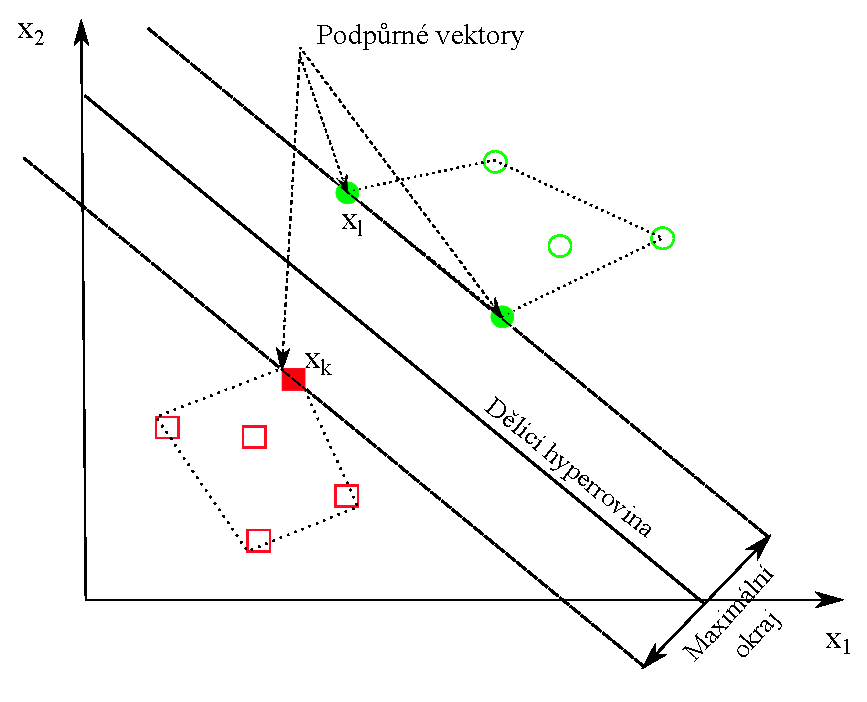
\includegraphics[width=0.63\linewidth]{figures/klasifikace/svm.eps}}
    \caption{Grafické znázornění oddělení vzorků dvou tříd pomocí hyperroviny. Vyplněné body, které tuto hyperrovinu definují, se nazývají podpůrné vektory.}
    \label{fig:svmObrazek}
\end{figure}

\begin{table}[H]
\begin{tabularx}{\linewidth}{>{\parskip1ex}X@{\kern4\tabcolsep}>{\parskip1ex}X}
\toprule
\hfil\bfseries Výhody
&
\hfil\bfseries Nevýhody
\\\cmidrule(r{3\tabcolsep}){1-1}\cmidrule(l{-\tabcolsep}){2-2}

Unikátní řešení\par
Nemá problém tzv. \emph{over-fitting} (česky přetrénování)\par
Velmi účinné\par
Poměrně nízká výpočetní složitost\par
Poskytuje flexibilitu v~možnosti výběru formy prahu
&
Vysoká složitost algoritmu a~s~tím spojená náročnost na pochopení\par
Poměrně pomalé trénování\par
Potíže s~nalezením optimálních parametrů při použití nelineárně odlišitelných dat


\\\bottomrule
\end{tabularx}
\caption{Výhody a~nevýhody metody SVM~\cite{classificMethodsComp2, classificMethodsComp3}.}
\end{table}


\subsection*{Umělé neuronové sítě}
\label{ANN}
Umělá neuronová síť je matematický model inspirovaný biologickými neuronovými sítěmi. Umělá neuronová síť se skládá se ze sekvence vrstev, kde každá vrstva se skládá z~propojené skupiny umělých neuronů a~zpracovává informace za použití přístupu založeného na těchto vazbách. Všechny neurony každé vrstvy jsou váhově spojeny s~neurony předchozí a~následující vrstvy, jak lze vidět na obrázku \ref{fig:ann}. Umělé neuronové sítě slouží pro vytváření složitých vztahů mezi vstupními a~výstupními daty. Úspěšnost těchto sítí závisí zejména na jejich struktuře a~počtu vstupů \cite{classificMethodsComp1, classificMethodsComp3, CVmodernApproach}.

Důležitá podmnožina umělých neuronových sítí pro obor zpracování obrazu jsou konvoluční neuronové sítě popsané samostatně v~kapitole \ref{detekceKonv}.

\begin{figure}[H]
    \centering
    \tmpframe{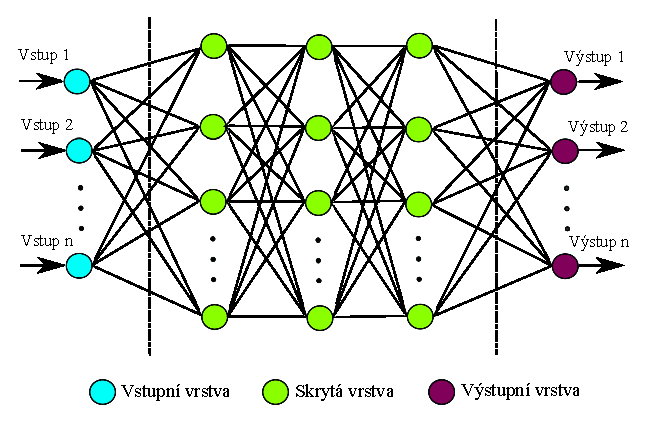
\includegraphics[width=0.70\linewidth]{figures/klasifikace/ann.eps}}
    \caption{Architektura umělé neuronové sítě se třemi skrytými vrstvami. Všechny neurony jsou váhově spojeny se všemi neurony předchozí a~následující vrstvy.}
    \label{fig:ann}
\end{figure}

Učení těchto sítí je možné rozdělit do dvou hlavních tříd:

\begin{itemize}
    \item \textbf{Metoda učení s~učitelem} Funguje na principu anotovaných (oštítkovaných) vstupních dat. Anotace reprezentují správný výsledek pro daný vstup. Pro každý vzorek tedy existuje vektor vstupních dat a~jeden či více očekávaných výsledků. Po provedení klasifikace je výsledek porovnán s~očekávaným výsledkem. Cílem této metody je snížit chybu klasifikace (pomocí ztrátové funkce).
    \item \textbf{Metoda učení bez učitele} se liší oproti metodě s~učitelem v~tom, že vstupní data nejsou vůbec anotovaná, tedy nejsou známy správné výstupy, pomocí kterých by se proces trénování řídil. Tyto sítě pracují na principu třídění vstupních dat na základě jejich podobnosti, bez možnosti ověření správnosti.
\end{itemize}

Většina úloh provádějící rozpoznání vzoru v~oboru zpracování obrazu je řešena pomocí první zmíněné metody učení s~učitelem \cite{CNN}.

\begin{table}[H]
\begin{tabularx}{\linewidth}{>{\parskip1ex}X@{\kern4\tabcolsep}>{\parskip1ex}X}
\toprule
\hfil\bfseries Výhody
&
\hfil\bfseries Nevýhody
\\\cmidrule(r{3\tabcolsep}){1-1}\cmidrule(l{-\tabcolsep}){2-2}

Velmi účinné pro velké datové sady\par
Odolné vůči šumu v~trénovací datové sadě\par
Bez-parametrický přístup. Tzn. nedělá předpoklady o~mapovací funkci\par
Vysoká výpočetní rychlost
&
Vysoká náročnost na výpočetní zdroje a~čas\par
Problém tzv. \emph{over-fitting} (česky přetrénování)\par
Složitost výběru/nalezení správné architektury


\\\bottomrule
\end{tabularx}
\caption{Výhody a~nevýhody umělých neuronových sítí~\cite{classificMethodsComp2, classificMethodsComp3}.}
\end{table}

\subsection*{Rozhodovací stromy}
\label{rozhodovaciStromy}
Rozhodovací strom~\cite{classificMethodsComp2, classificMethodsComp3} vytváří stromovou strukturu jednotlivých rozhodnutí. Rozhodnutí o~členství v~třídě je provedeno pomocí opakovaného rozdělování vstupní datové sady do jednotlivých podmnožin. Je to metoda učení s~učitelem a~oproti umělým neuronovým sítím je bezparametrická. Každá větev graficky znázorňuje rozhodnutí, které by mělo být vykonáno. Metoda umožňuje rozhodnutí o~třídě (akceptaci či odmítnutí) v~libovolném mezikroku a~po provedení klasifikace při trénování rozhodovací stromy udávají sadu pravidel, která by měla být modelem zapamatována. Metoda se skládá ze třech částí. První je rozdělení jednotlivých uzlů, poté následuje nalezení listových uzlů a~nakonec přidělení tříd jednotlivým listovým uzlům.

Metodu rozhodovacích stromů lze ještě dále rozšířit pomocí metody zvané \emph{Random forest} (náhodný les), která během procesu trénování vytváří množinu několika rozhodovacích stromů, kde každý udává (hlasuje pro) třídu vstupního vzorku.

\begin{figure}[H]
    \centering
    \tmpframe{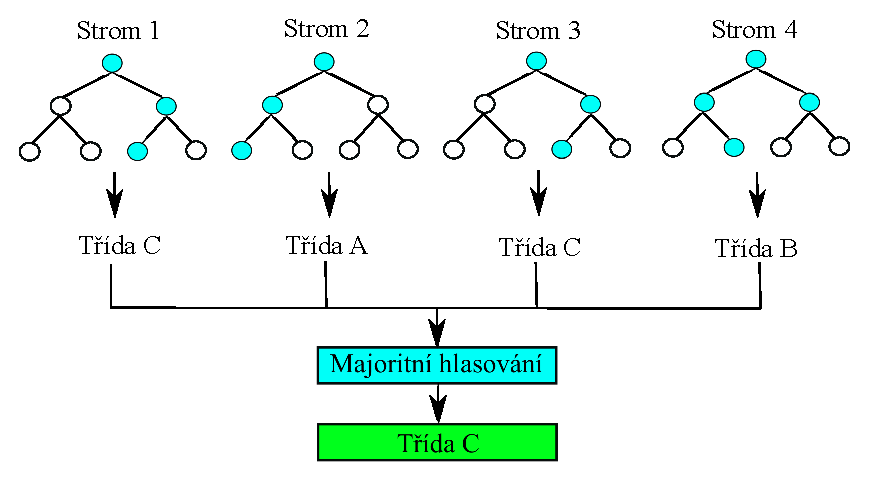
\includegraphics[width=0.7\linewidth]{figures/klasifikace/randomForest.eps}}
    \caption{Náhodný les složený ze čtyř rozhodovacích stromů.}
    \label{fig:rozhodStromy}
\end{figure}

Výsledná třída je určena na základě výsledků jednotlivých rozhodovacích stromů a~to tak, že je vybrána třída s~nejvyšším počtem hlasů \cite{classificMethodsComp1}, znázorněno na obrázku \ref{fig:rozhodStromy}.

\begin{table}[H]
\begin{tabularx}{\linewidth}{>{\parskip1ex}X@{\kern4\tabcolsep}>{\parskip1ex}X}
\toprule
\hfil\bfseries Výhody
&
\hfil\bfseries Nevýhody
\\\cmidrule(r{3\tabcolsep}){1-1}\cmidrule(l{-\tabcolsep}){2-2}

Jednoduché na pochopení\par
Bez-parametrický přístup\par
Nízká výpočetní náročnost
&
Vysoká míra chybovosti klasifikace\par
Rozdělení je velmi citlivé vůči trénovací datové sadě

\\\bottomrule
\end{tabularx}
\caption{Výhody a~nevýhody rozhodovacích stromů~\cite{classificMethodsComp2, classificMethodsComp3}.}
\end{table}



%%%%%%%%%%%%%%%%%%%%%%%%%%%%%%%%%%%%%%%%%%%%%%%%%%%%%%%%%%%%%%%%%%%%%%%%%%%%%%%%%%%%%%%%%%%


\section{Vyhodnocení úspěšnosti detekce}
\label{vyhodnoceniUspesnosti}
Ve chvíli, kdy už existuje funkční model pro detekci objektů, je dobré vyhodnotit jeho úspěšnost. Úspěšnost detekce ve většině případů nestačí vyhodnotit pouhým pozorováním detekovaných obrázků (tedy kvalitativně), ale vyjadřuje se kvantitativně -- proto je potřeba si zavést pojmy, které usnadní validaci detekcí a~určení celkové kvality detektoru. Při studiu této problematiky jsem vycházel z~\cite{mAP}.

\subsection*{Intersection over union -- IoU}
\emph{Intersection over union} (dále jen mezi odborníky běžně používaná zkratka IoU), se počítá na základě dvou ohraničujících boxů -- \emph{ground-truth} (požadovaná výstupní hodnota, dále bude používán jen anglický tvar) -- tedy pozice kde se objekt nachází a~predikce vytvořené detektorem. IoU udává překrytí predikce a~ground-truth normalizované na hodnotu náležící do intervalu $\langle0,1\rangle$. Vizualizováno na obrázku \ref{fig:priou}.

\subsection*{Typy predikcí}
Predikce detektoru jsou rozděleny do čtyř následujících tříd, dále budou požívány pouze jejich zkratky.

\begin{enumerate}
    \item \textbf{True positive} -- Udává správně detekovaný objekt (IoU je větší než hodnota prahu).
    \item \textbf{False positive} -- Udává špatně detekovaný objekt (IoU je menší než hodnota prahu).
    \item \textbf{False negative} -- Udává nedetekovaný objekt.
    \item \textbf{True negative} -- Místa kde není objekt jsou správně označena jako bez-objektová (používá se výjimečně).
\end{enumerate}


\subsection*{Precision}
\emph{Precision} (přesnost, nadále bude využívána jen anglická forma, protože to je zvykem i~mezi odborníky v~oboru), udává, jak přesné predikce jsou. Běžně se uvádí v~procentech a~vyjadřuje kolik z~predikcí je pravdivých:
\begin{align}
    \label{eq:precision}
    \mathrm{Precision} &= \frac{\mathrm{TP}}{\mathrm{TP} + \mathrm{FP}}
\end{align}
\subsection*{Recall}
\emph{Recall} (citlivost, nadále bude využívána jen anglická forma, protože to je zvykem i~mezi odborníky v~oboru), udává, kolik ze všech pozitivních případů bylo správně predikováno:
\begin{align}
    \label{eq:recall}
    \mathrm{Recall} &= \frac{\mathrm{TP}}{\mathrm{TP} + \mathrm{FN}}
\end{align}
\begin{figure}[H]
    \centering
    \tmpframe{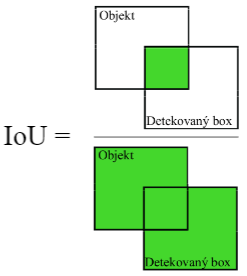
\includegraphics[width=0.3\linewidth]{figures/klasifikace/iou.png}}
    \caption{Grafické znázornění IoU pomocí predikovaného a \emph{ground-truth} boxu.}
    \label{fig:priou}
\end{figure}    

\subsection*{Average precision -- AP}
\emph{Average precision} (dále jen mezi odborníky běžně používaná zkratka AP), je metrika používaná pro měření přesnosti detektoru objektů. Udává průměr maximálních hodnotu precision pro různé hodnoty recall. Princip AP je konceptuálně stejný jako počítání plochy pod precision-recall křivkou (AuC -- \emph{area under curve}). První je ale potřeba tzv. vyhladit křivku. Toho se dosáhne interpolací. Vytvoří se graf s~hodnotou recall \Tilde{r} $0.0, 0.1, ... 1.0$ a~každá hodnota precision se nahradí maximální hodnotou precision pro recall $\geq \Tilde{r}$. Graficky znázorněno na obrázku \ref{fig:prcurve}.

\begin{figure}[H]
    \centering
    \tmpframe{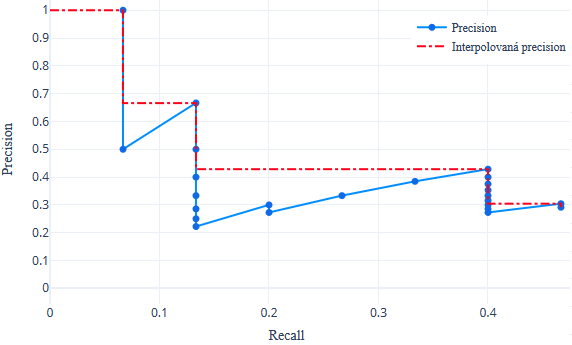
\includegraphics[width=0.75\linewidth]{figures/klasifikace/prcurve.png}}
    \caption{Precission-recall křivka a~její interpolace.}
    \label{fig:prcurve}
\end{figure}

AP je počítáno jako průměr maximálních hodnot precision na jedenácti hodnotách recall $(0.0, 0.1, ... 1.0)$. Záměrem interpolace křivky na jedenácti bodech je snížit dopad \uv{zákmitů} křivky, způsobených malými odchylkami hodnocení vzorků. Výpočet je následující:
\begin{align}
    \label{eq:map}
    \mathrm{AP} &= \frac{1}{11} \sum\limits_{r \in \{0.0,...,1.0\}} AP_r\\ &= \frac{1}{11} \sum\limits_{r \in \{0.0,...,1.0\}} p_{i}(r)
\end{align}
kde
\begin{align}
    \label{eq:interpol}
    p_{i}(r) = \max\limits_{\Tilde{r} \geq r} p(\Tilde{r})
\end{align}
Hodnota $p_{i}$ značí interpolovanou precision. AP se počítá pro každou třídu zvlášť, proto se u~detektorů běžně používá mAP (\emph{mean average precision}), což je průměr AP všech tříd.


%%%%%%%%%%%%%%%%%%%%%%%%%%%%%%%%%%%%%%%%%%%%%%%%%%%%%%%%%%%%%%%%%%%%%%%%%%%%%%%%%%%%%%%%%%%


\section{Související práce}
\label{existujiciReseni}
Detekce a~klasifikace dopravních značek je již mnoho let řešená problematika, které spadá do dynamicky rozvíjejícího se oboru detekce objektů v~obraze. Existuje velké množství přístupů k~řešení této problematiky, ale i~přesto detekce značek stále není považována za úplně vyřešenou a~vznikají nové práce, jako je například tato, provádějící detekci za pomoci moderních technik ve snaze posunout tuto problematiku vpřed.

Porovnání výsledků jednotlivých prací není jednoduché, protože se často liší použitými metrikami pro vyhodnocení (hit rate, mAP (interpolovaná), mAP@0.5, mAP@0.75, ROC, F1, atd.). Dalším faktorem při vyhodnocení, který má poměrně velký vliv na celkovou úspěšnost, je použitá datová sada -- datové sady se liší ať už konvencí značek, tak zejména jejich kvalitou a kvantitou. Jejich přehled je možné najít v~sekci~\ref{datoveSady}.

Jak plyne z~porovnání detekčních metod dopravních značek~\cite{tsDetectOverview}, dříve byla tato úloha řešena pomocí segmentace obrazu na základě barvy v~kombinaci s~detekcí geometrických útvarů či rohů~\cite{tsDetect}. V~práci~\cite{fastShapeTSD} se autoři zabývali rychlou metodou detekce tvarů založenou na Houghově transformaci přímo pro detekci dopravních značek. Výsledkem byla $95\,\%$ úspěšnost detekce a~metoda je navíc invariantní vůči natočení značky a~pracuje v~reálném čase.

Metoda hojně využívaná pro detekci značek je extrakce příznaků z~obrazu v~kombinaci s~klasifikátorem. Před příchodem konvolučních neuronových sítí byl přístup s~použitím histogramu orientovaných gradientů (dále jen HOG) v~kombinaci s~SVM (\emph{Support Vector Machines}) označován za tzv. \emph{state of the art}\footnotemark \, detekce objektů~\cite{tsdYolo}. V~práci~\cite{tsdHog} využívající zmíněnou kombinaci HOG a~SVM se podařilo získat na Německé datové sadě výsledky detekce značek s~hodnotami \emph{precision} i~\emph{recall} blížícími se k~jedné, ale vyhodnocení jednoho snímku trvalo déle než vteřinu. Další možností je použití metody využité v~práci~\cite{tsdHaar} -- kombinaci Haarových příznaků s~lineárním SVM pro klasifikaci (a konvolučními neuronovými sítěmi pro verifikaci), pomocí které se podařilo na Německé datové sadě dosáhnout taktéž výsledků s~hodnotami \emph{precision} i~\emph{recall} blížícím se k~jedné a~zároveň zpracování v~reálném čase.

\footnotetext{\emph{State of the art} -- stav techniky (tzn. aktuálně nejlepší způsob pro řešení dané problematiky).}

V~posledních letech přitáhlo velkou pozornost hluboké učení a~standardem pro detekci objektů se tak staly konvoluční sítě. Práce~\cite{rcnn} prokázala, že jejich použití pro detekci objektů může vést ke dramatickému zvýšení úspěšnosti detekce. Výborných výsledků detekce objektů dosáhla metoda R-CNN, která kombinuje návrh kandidátních oblastí (selektivní hledání~\cite{selective-search}) s~konvolučními sítěmi a~řadí se tak do třídy dvou-krokových metod. Upravená verze této metody, Faster R-CNN, byla použita v~práci~\cite{tsdFastRcnn} pro detekci značek a~dosáhla úspěšnosti $34.4\,\%$ mAP na Belgické datové sadě.

Pro rychlejší, ale stále přesnou detekci vznikla třída tzv. \emph{single-shot} detektorů, kam spadá YOLO a~SSD (\emph{Single Shot Detector}). Ty provádí detekci i~klasifikaci pomocí jedné konvoluční sítě. Upravený systém Tiny YOLOv1 byl pro detekci značek použit v~práci~\cite{tsdYolo}, kde se autorům podařilo dosáhnout úspěšnosti $33.8\,\%$ mAP na Belgické datové sadě dopravních značek s~rychlostí 100 snímků za sekundu. SSD byl použit v~práci~\cite{tsdSsd}, kde se autoři snažili o~přesný odhad okrajů dopravních značek a~dosáhli úspěšnosti kolem $85\,\%$ mAP na Německé datové sadě při rychlosti 7 snímků za sekundu na zařízení s poměrně nízkým výpočetním výkonem.

Z~dosažených výsledků zmíněných prací vyplývá, že pro úlohu detekce dopravních značek stále dosahují lepší úspěšnosti systémy využívající extrakci příznaků v~kombinaci s~klasifikátorem, ale konvoluční sítě je pomalu dohánějí jak z~hlediska úspěšnosti, tak rychlosti.


\chapter{Detekce pomocí konvolučních neuronových sítí}
\label{detekceKonv}
Konvoluční neuronové sítě existují již řadu let, ale standardem pro úlohy rozpoznání vzoru v~oboru zpracování obrazu se staly až v~posledních letech. Je to zapříčiněno zejména vyšším výpočetním výkonem počítačů a~velkému množství obrázků a~jimi tvořených datových sad, na kterých je možné tyto neuronové sítě trénovat.

%%%%%%%%%%%%%%%%%%%%%%%%%%%%%%%%%%%%%%%%%%%%%%%%%%%%%%%%%%%%%%%%%%%%%%%%%%%%%%%%%%%%%%%%%%%

\section{Konvoluční neuronové sítě}
\label{cnnTeorie}
Při studiu jsem vycházel z~\cite{CNN, CVmodernApproach}. Hlavní rozdíl mezi konvolučními a~klasickým umělými neuronovými sítěmi je v~tom, že konvoluční sítě jsou používány zejména pro účely rozpoznání vzorů v~oboru zpracování obrazu. Největší nevýhodou umělých neuronových sítí pro výpočet obrazových dat je jejich problém s~vysokou výpočetní složitostí -- dokáží si poradit pouze s~obrázky s~jedním kanálem a~malým rozlišením. Pro komplexnější obrazové vstupy by taková neuronová síť byla příliš velká pro efektivní učení.

\subsection*{Architektura}
Konvoluční neuronové sítě se skládají ze třech typů vrstev. Konvolučních, pooling (sdružovacích) a~plně propojených. První vrstva se nazývá vstupní a~poslední výstupní, mezi nimi se nacházejí vrstvy skryté. Podle \cite{CNN} je postup zpracování jednoho snímku následovný:

\begin{enumerate}
	\item Hodnoty jednotlivých pixelů snímku se uloží do vstupní vrstvy
	\item \textbf{Konvoluční vrstva} určí hodnoty jednotlivých neuronů. Ty jsou dány konvolucí jádra (vah) a~lokální části vrstvy (zvané jako receptivní pole neuronu), se kterou je neuron spojen. Přenosová funkce umístěná za konvoluční vrstvou (např. ReLU\footnotemark) slouží k~provedení aktivací pro každý prvek z~předchozí vrstvy.
	\footnotetext{ReLU -- \emph{Rectified Linear Unit} (rektifikovaná lineární jednotka).}
	\item \textbf{Sdružovací vrstva} poté provede tzv. \emph{downsampling}, tedy podvzorkování (snížení počtu vzorků -- informace), a~to buď za pomoci maximalizace či průměrování okolí pixelu a~výsledkem je pouze jedna hodnota. To slouží ke zmenšení velikosti dané vrstvy.
	\item \textbf{Konvoluční} a \textbf{sdružovací} vrstvy se mohou opakovat. Hluboké konvoluční neuronové sítě se zpravidla skládají z několika skrytých konvolučních vrstev.
	\item Nakonec \textbf{plně-propojená vrstva} vyprodukuje skóre (pravděpodobnosti) jednotlivých tříd z aktivací, sloužící ke klasifikaci.
\end{enumerate}

Proces zpracování konvoluční neuronovou sítí popsaný výše lze vidět na obrázku \ref{fig:cnn}. Díky této jednoduché transformaci dokáže konvoluční neuronová síť za pomoci konvolučních a~podvzorkovacích technik převést vstupní obrázek z~matice pixelů na skóre jednotlivých tříd pro účely klasifikace či regrese.

\begin{figure}[H]
    \centering
    \tmpframe{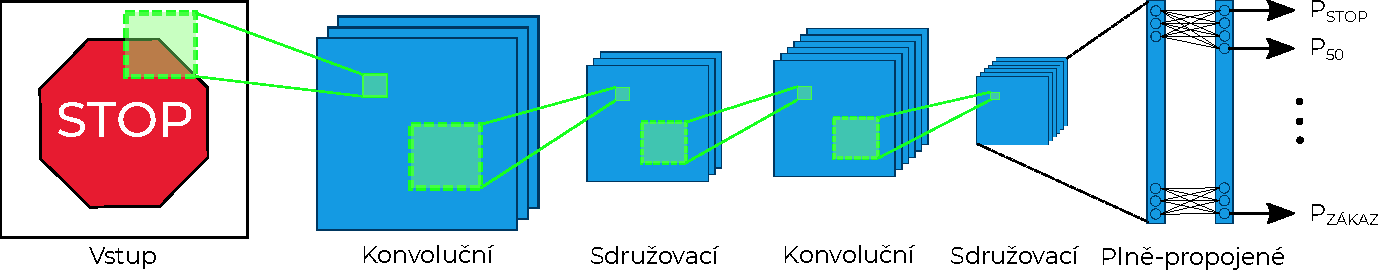
\includegraphics[width=0.99\linewidth]{figures/cnn/CNN.pdf}}
    \caption{Základní architektura konvoluční neuronové sítě.}
    \label{fig:cnn}
\end{figure}

\subsection*{Konvoluční vrstva}
Konvoluční vrstvy sehrávají ve fungování celé konvoluční neuronové sítě nezastupitelnou roli. Parametry jednotlivých vrstev jsou založeny na \uv{učících} se jádrech. Tato jádra jsou ve své podstatě matice, běžně o~malém rozměru. Ve chvíli, kdy se data dostanou do konvoluční vrstvy, je postupně prováděna konvoluce všech jader se vstupními daty. Protože jsou vstupní data dvou-rozměrná, lze pomocí jednotlivých konvolučních jader \uv{přejíždět} přes vstupní data a~produkovat výsledek této operace jako jednu hodnotu, jak lze vidět na obrázku \ref{fig:cnnKonvoluce}. Výstupem je poté tzv. \emph{heat map} (česky zvaná aktivační mapa), zobrazená na obrázku \ref{fig:cnnHeatMap}. Postupným učením se jádro zlepšuje a~poté, když ve vstupu na jisté pozici najde určitou vlastnost, vydá podnět známý jako aktivace \cite{CNN}.

Pomocí optimalizace výstupu dokáže konvoluční vrstva také snížit celkovou složitost modelu. Tato optimalizace se provádí za pomoci třech hyper-parametrů, zvaných \emph{depth} (hloubka), \emph{stride} (krok), a~\emph{zero-padding} (nulové vyplňování). Hloubku lze nastavit pomocí počtu neuronů uvnitř vrstvy. Snížením tohoto hyper-parametru lze docílit podstatně nižšího počtu neuronů v~síti, a~tedy složitosti, ale zároveň se tím sníží schopnost rozpoznání vzorů. Krok určuje, o~kolik se jádro posouvá při provádění konvolucí jader se vstupními daty. Při nastavení kroku na jedna by se receptivní pole jednotlivých neuronů příliš překrývala a~výsledkem by byly příliš velké aktivace. Naopak při nastavení kroku na číslo velké by znamenalo velké mezery mezi receptivními poli neuronů a~tedy příliš malé rozměry výstupu. Nulová výplň je technika vyplňování krajů vstupu a~poskytuje vyšší kontrolu rozměrů výstupu. Pomocí těchto parametrů je tedy možné změnit dimenze výstupů a~jejich výpočet je následující \cite{CNN}:
\begin{align}
    \label{eq:cnn}
    D &= \frac{(V - R) + 2Z}{S + 1}
\end{align}
Kde $R$ udává velikost receptivního pole neuronu (stejné jako velikost jádra), $S$ udává krok, $V$ udává velikost vstupu (tedy výška $\times$ šířka $\times$ hloubka) a~$Z$ je velikost nulové výplně.

\begin{figure}[!htb]
    \centering
    \begin{minipage}{.5\textwidth}
      \centering
      \tmpframe{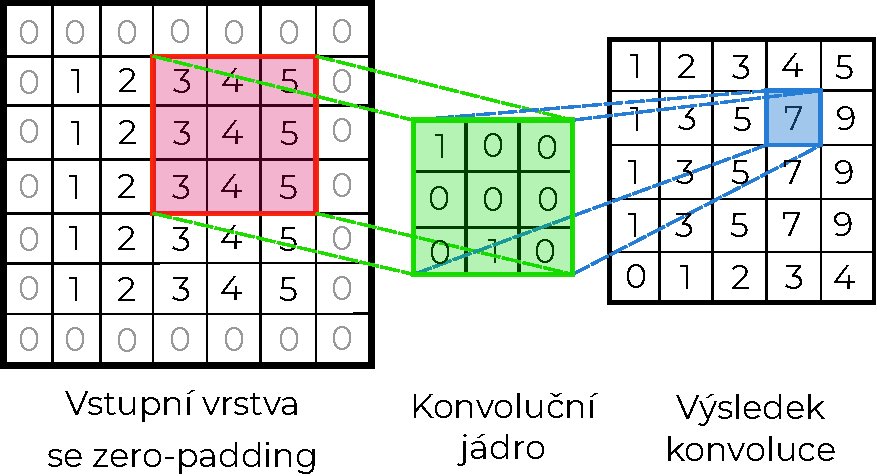
\includegraphics[width=0.99\linewidth]{figures/cnn/konvoluce.pdf}}
      \caption{Konvoluce vstupu velikosti $5\times5$ (se \emph{zero-padding} rovno jedné) s~jádrem \\ o velikosti $3\times3$.}
      \label{fig:cnnKonvoluce}
    \end{minipage}%
    \begin{minipage}{.5\textwidth}
      \centering
      \tmpframe{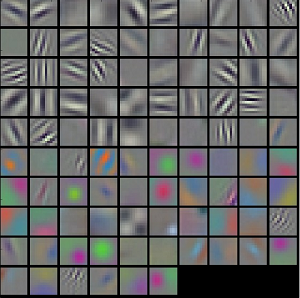
\includegraphics[width=0.67\linewidth]{figures/cnn/cnnHeatMap.png}}
      \caption{Aktivační mapy pocházející z první konvoluční vrstvy.\footnotemark}
      \label{fig:cnnHeatMap}
    \end{minipage}%
\end{figure}

Vytváření architektury konvoluční neuronové sítě je složitý proces a~existují tu jisté ověřené metody. Běžná architektura těchto sítí je založena na tom, že každá konvoluční vrstva je následována vrstvou sdružovací a~to se opakuje až po plně propojenou vrstvu. Pro rozpoznání složitějších vlastností v~obraze je doporučeným postupem umístit za sebe několik konvolučních vrstev. Dalším ověřeným postupem je rozdělení jedné velké konvoluční vrstvy na několik menších, což slouží pro snížení výpočetní náročnosti pro danou konvoluční vrstvu \cite{CNN}.

\footnotetext{Převzato z~\url{http://cs231n.github.io/understanding-cnn}.}


\subsection*{Overfitting}
\emph{Overfitting}, český zvané \uv{přetrénování} znamená, že neuronová síť se už nedokáže efektivně učit. Nastává ve chvíli, kdy neuronová síť dokáže správně predikovat pouze obrázky z~trénovací datové sady, ale selhává u~všech ostatních. Řešením je například snížení počtu parametrů, které je třeba se naučit. Čím méně parametrů je třeba se naučit, tím menší je pravděpodobnost výskytu přetrénování \cite{CNN}.

%%%%%%%%%%%%%%%%%%%%%%%%%%%%%%%%%%%%%%%%%%%%%%%%%%%%%%%%%%%%%%%%%%%%%%%%%%%%%%%%%%%%%%%%%%%


\section{You Only Look Once -- YOLO}
\label{yoloTeorie}
Při studiu této problematiky jsem vycházel z~\cite{yolov1,yolo9000,yolov3,yolov3_article,yolov123,tsdYolo}. Systém YOLO přistupuje k~detekci objektů jako k~jednotné regresi, přímo od pixelů snímku k~souřadnicím ohraničujících boxů a~pravděpodobnostem jednotlivých tříd. Systém YOLO je poměrně jednoduchý, za pomoci jediné konvoluční neuronové sítě predikuje množinu ohraničujících boxů a~zároveň pravděpodobnosti tříd. YOLO je speciální systém, který je trénovaný na tzv. \uv{plných obrázcích} (tedy celých snímcích, nikoli vyřezaných objektech jako klasifikátory) a~při tom rovnou optimalizuje úspěšnost detekce. Tento systém má oproti běžným přístupům detekce objektů řadu výhod.

Zaprvé, YOLO přistupuje k~detekci jako k~regresnímu problému, což umožňuje odstranění složité \emph{pipe-line} (posloupnost kroků). To umožňuje provádět detekce velmi rychle při zachování dobré úspěšnosti. Základní verze YOLO pracuje na rychlosti zpracování 45 snímků za sekundu a~odlehčená verze dokonce na více než 150 snímcích za sekundu na grafickém čipu Titan X. YOLO také dosahuje více než dvojnásobek mAP než ostatní \emph{real-time} detektory (detektory, které dokáží pracovat v~reálném čase).

Zadruhé, YOLO na rozdíl od metod posuvného okna a~návrhu oblastí (\emph{region-proposal}) během trénování i~testování \uv{vidí} celý snímek, což tomuto systému umožňuje se naučit kontextuální informace o~třídách, stejně jako jejich vzhled. Metoda R-CNN popsaná v~sekci~\ref{rcnnTeorie} (jeden z nejúspěšnějších systémů pro detekci) zaměňuje velké množství částí pozadí za objekty, protože nevidí širší kontext, ve kterém se objekty nachází.

Zatřetí, YOLO se učí obecnou reprezentaci objektů. Například pokud je natrénováno na přirozených obrázcích a~vyhodnoceno na umění, dosahuje mnohem lepších výsledků než ostatní detekční systémy. To znamená mnohem nižší pravděpodobnost selhání při neočekávaném či úplně jiném typu vstupu \cite{yolov1}.


\subsection*{Princip fungování systému YOLO}
Systém rozděluje vstupní snímek na mřížku o~velikosti $S \times S$ buněk, jak lze vidět na obrázcích~\ref{fig:YOLO_1}~a~\ref{fig:YOLO_2}. Pokud se střed objektu nachází v~buňce, pak je daná buňka zodpovědná za detekci tohoto objektu.

Každá buňka predikuje $B$ ohraničujících boxů a~zároveň také jistotu (angl. \emph{confidence}), s~jakou dané boxy predikuje. Tyto jistoty udávají, jak si je model jistý, že daný box obsahuje objekt (anglicky tzv. \emph{objectness} -- dále jen objektovost), a~také jak přesný box je. Tuto jistotu lze formálně definovat jako $\text{Pr(Object)} \times \text{IoU}_{\text{pred}}^\text{truth}$, kde $\text{Pr(Object)}$ udává pravděpodobnost výskytu objektu v boxu a $\text{IoU}_{\text{pred}}^\text{truth}$ udává IoU mezi predikovaným a \emph{ground-truth} boxem. Pokud se v~dané buňce žádný objekt nenachází, mělo by skóre objektovosti být ideálně rovno nule, v~opačném případě rovno IoU mezi boxy predikce a~\emph{ground-truth}.

Každý ohraničující box je složen z~pěti predikcí. Jmenovitě to jsou $x,y,w,h$ a~jistota boxu. Souřadnice $x$,$y$ reprezentují střed predikovaného boxu, $w$ a~$h$ pak výšku a~šířku daného boxu. Tyto hodnoty jsou relativní (normalizovány velikostí celého obrázku). Poslední predikce, jistota boxu, udává IoU mezi predikovaným a~kterýmkoli \emph{ground-truth} boxem.

Každá buňka také predikuje $C$ podmíněných pravděpodobností jednotlivých tříd -- $\text{Pr(Class}_{i}\text{|Object)}$. Tyto pravděpodobnosti jsou podmíněny tím, zda se v~dané buňce nachází objekt. Predikováno je takové množství sad pravděpodobností všech tříd, jaký je počet buněk, nezávisle na počtu predikovaných ohraničujících boxů.

\begin{figure}[H]
    \centering
    \tmpframe{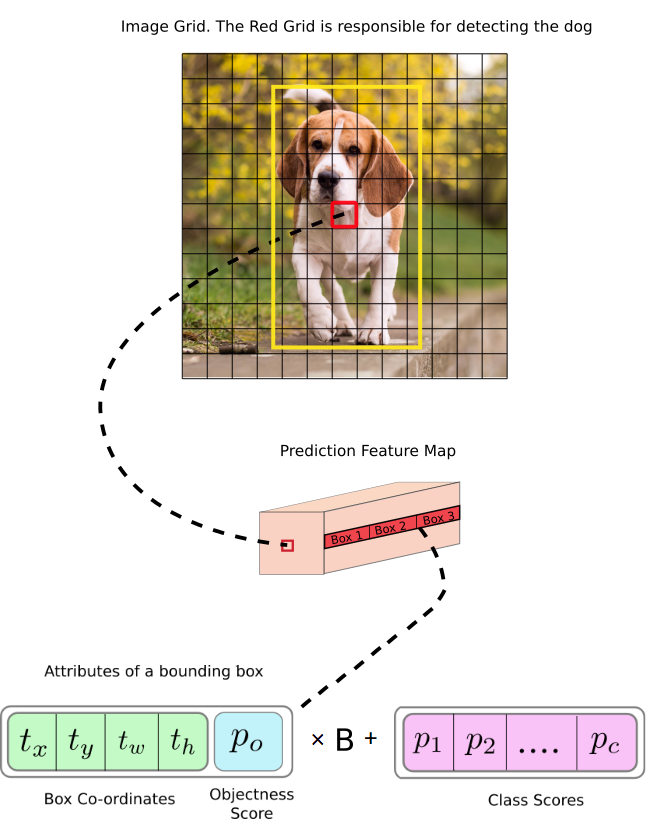
\includegraphics[width=0.6\linewidth]{figures/cnn/yolo_1.png}}
    \caption{Princip vytváření predikcí pomocí systému YOLO. Výsledkem je tenzor o~velikosti $S\times S\times(B\times 5 + C)$.\footnotemark}
    \label{fig:YOLO_1}
\end{figure}

\footnotetext{Převzato z~\url{https://blog.paperspace.com/how-to-implement-a-yolo-object-detector-in-pytorch} a~upraveno.}

Při testování se násobí podmíněné pravděpodobnosti tříd s~jistotou predikce jednotlivých boxů:
\begin{align}
    \label{eq:yolo}
    \text{PR(Class}_{i}\text{|Object)} \times \text{Pr(Object)} \times \text{IoU}_{\text{pred}}^\text{truth} = \text{PR(Class}_{i}\text{)} \times \text{IoU}_{\text{pred}}^\text{truth},
\end{align}
což udává jistotu jednotlivých tříd pro každý ohraničující box. Tato skóre udávají jak pravděpodobnost, že se třída v~daném boxu nachází, tak jak dobře ohraničuje predikovaný box daný objekt. Vizualizováno na obrázku \ref{fig:YOLO_2}.

\begin{figure}[H]
    \centering
    \tmpframe{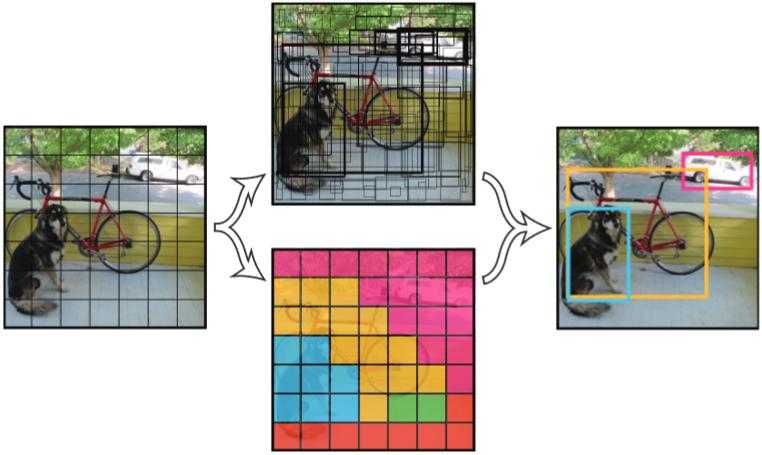
\includegraphics[width=0.75\linewidth]{figures/cnn/yolo_2.png}}
    \caption{Vytvoření prediktivních ohraničujících boxů. Tloušťka hrany boxu reprezentuje jistotu, s~jakou systém daný objekt predikuje -- čím tlustější, tím si je systém jistější.\footnotemark}
    \label{fig:YOLO_2}
\end{figure}

\footnotetext{Převzato z~\cite{yolov1}.}


\subsection*{Architektura}
Architekturu základní verze systému YOLO je možné vidět na obrázku \ref{fig:YOLO_3}. Skládá se ze 24 konvolučních vrstev následovaných dvěma plně-propojenými vrstvami. Střídající se vrstvy o~velikosti $1 \times 1$ slouží pro snížení množství vlastností z~předcházejících vrstev. Počáteční vrstva slouží k~extrakci vlastností ze vstupních snímků a~koncové plně-propojené vrstvy slouží k~predikci výstupních pravděpodobností jednotlivých tříd a~souřadnic ohraničujících boxů. Výstupem je tenzor predikcí o~velikosti $7 \times 7 \times 30$.

\begin{figure}[H]
    \centering
    \tmpframe{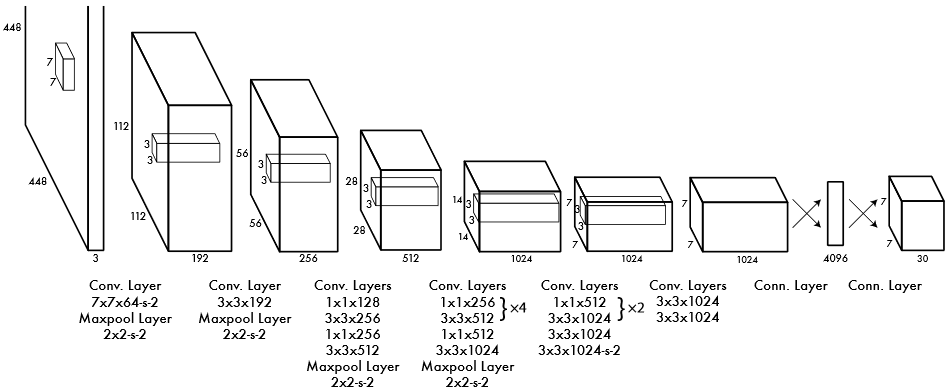
\includegraphics[width=0.8\linewidth]{figures/cnn/yolo_3.png}}
    \caption{Architektura základní verze YOLO.\footnotemark}
    \label{fig:YOLO_3}
\end{figure}

\footnotetext{Převzato z~\cite{yolov1}.}

\subsection*{Ztrátová funkce}
Systém YOLO vytváří několik predikcí pro každou buňku mřížky, ale pouze jedna z~nich je zodpovědná za predikci objektu, a~to ta s~nejvyšším IoU s~\emph{ground-truth}. Ztrátová funkce slouží k~ověření, jak dobře systém odpovídá trénovací sadě. Při trénování pomocí systému YOLO je optimalizována ztrátová funkce skládající se z~několika následujících částí.
\begin{align}
\mathrm{Loss} = &\lambda_{coord} \sum_{i=0}^{S^2}\sum_{j=0}^B \mathds{1}_{ij}^{obj}[(x_i-\hat{x}_i)^2 + (y_i-\hat{y}_i)^2 ] \label{eq:yoloLoss_1}\\
&+ \lambda_{coord} \sum_{i=0}^{S^2}\sum_{j=0}^B \mathds{1}_{ij}^{obj}[(\sqrt{w_i}-\sqrt{\hat{w}_i})^2 +(\sqrt{h_i}-\sqrt{\hat{h}_i})^2 ]\label{eq:yoloLoss_2}\\
&+ \sum_{i=0}^{S^2}\sum_{j=0}^B \mathds{1}_{ij}^{obj}(C_i - \hat{C}_i)^2 \label{eq:yoloLoss_3}\\
&+ \lambda_{noobj}\sum_{i=0}^{S^2}\sum_{j=0}^B \mathds{1}_{ij}^{noobj}(C_i - \hat{C}_i)^2 \label{eq:yoloLoss_4}\\
&+ \sum_{i=0}^{S^2} \mathds{1}_{i}^{obj}\sum_{c \in classes}(p_i(c) - \hat{p}_i(c))^2 \label{eq:yoloLoss_5}
\end{align}
kde $\mathds{1}_{i}^{obj} = 1$ pokud se v~buňce $i$ nachází objekt, jinak $0$. Dále pak $\mathds{1}_{ij}^{obj} = 1$ udává, že $j$-tý ohraničující box je zodpovědný za detekci v~rámci buňky $i$. Systém YOLO používá tzv. \emph{sum-squared error} mezi predikovanými a~\emph{ground-truth} boxy a~třídami. Funkce se dá rozdělit na pět částí, penalizující systém za tři typy chyb.

\begin{itemize}
    \item \textbf{Chyba klasifikace} -- Prochází každou buňku mřížky a~pokud se v~ní nachází objekt, tato chyba je vypočítána jako \emph{squared-error} podmíněné pravděpodobnosti třídy, a~to pro všechny třídy pomocí rovnice \eqref{eq:yoloLoss_5}. Pravděpodobnost výskytu třídy~$c$ v~buňce~$i$~ud- ává $\hat{p}_i(c)$.
    \item \textbf{Chyba lokalizace} -- Tato chyba udává, jak dobře či špatně byl objekt lokalizován, tedy rozdíl souřadnic a~velikosti predikovaného boxu vůči \emph{ground-truth} pomocí rovnic~\eqref{eq:yoloLoss_1}~a~\eqref{eq:yoloLoss_2}. Ke zvýšení váhy chyby predikce souřadnic ohraničujícího boxu slouží~$\lambda_{coord}$.
    \item \textbf{Chyba jistoty predikce} -- Pokud je v~boxu detekován objekt, tak se tato chyba počítá pomocí rovnice \eqref{eq:yoloLoss_3}, jinak \eqref{eq:yoloLoss_4}. Většina boxů neobsahuje objekt, což způsobuje nevyváženost, a~proto $\lambda_{noobj}$ snižuje váhu chyby při detekci pozadí.
\end{itemize}

\subsection*{Non-maxima suppression}
Systém YOLO může vytvořit duplicitní predikce jednoho objektu, proto provádí \emph{non-maxima suppression} (potlačení ne-maximálních hodnot) k~odstranění predikcí s~nižší jistotou, což může vést ke zvýšení mAP až o~$3\,\%$~\cite{yolov123}. Běžná implementace tohoto potlačení je následovná:

\begin{enumerate}
    \item Seřadit predikce podle jistoty.
    \item Začít procházet predikce od těch s~nejvyšší jistotou a~ignorovat všechny predikce, které mají stejnou třídu a~$\text{IoU} > 0.5$ s~aktuální predikcí.
    \item Opakovat krok 2 dokud nejsou všechny predikce zkontrolovány.
\end{enumerate}

\subsection*{Odlehčená verze -- Tiny YOLO}
\label{tinyToloTeorie}
Odlehčená verze, zvaná Tiny či Fast YOLO, se skládá z~menšího počtu konvolučních vrstev (9 oproti 24) a~také méně filtrů v~těchto vrstvách než základní verze. Kromě zmíněné změny velikosti jsou všechny ostatní parametry jak při trénování, tak testování u~odlehčené verze zachovány. Architektura odlehčené verze je navržena tak, aby posunula hranice rychlé detekce objektů. Jak již bylo zmíněno, dosahuje rychlosti zpracování více než 150 snímků za sekundu na GPU Titan X (oproti základní verzi, která zvládne zpracovat 45 snímků za sekundu) \cite{yolov1, yolov123}.


\subsection*{Třetí generace architektury -- YOLOv3}
\label{yolov3Teorie}
Třetí verze YOLO (dále jen YOLOv3) provádí predikce boxů na \textbf{třech různých rozměrech}, které jsou dány zmenšením dimenzí vstupního obrazu o~32, 16 a~8, jak lze vidět na obrázku \ref{fig:YOLOv3}. Systém získává z~různým rozměrů snímku vlastnosti pomocí konceptu podobného tzv. \emph{feature pyramid networks}. K~extraktoru vlastností z~původní verze YOLO je přidáno několik dalších konvolučních vrstev. Poslední z~těchto vrstev predikuje 3D tenzor obsahující ohraničující box, objektovost (s~jakou jistotou se v~boxu nachází objekt) a~pravděpodobnosti jednotlivých tříd. Základní verze YOLO měla problém s~detekcí malých objektů. Za pomoci predikce na různých rozlišeních má nyní YOLOv3 relativně \textbf{dobrou úspěšnost detekce malých objektů}, ale na druhou stranu se u~této verze snížila úspěšnost detekce středně velkých a~velkých objektů. Třetí verze obecně dosahuje lepších výsledků detekce než předchozí verze, a~to za cenu snížení rychlosti detekce. Změny se také dočkala ztrátová funkce, kde byla v~posledních třech částech (rovnice \eqref{eq:yoloLoss_3}, \eqref{eq:yoloLoss_4} a \eqref{eq:yoloLoss_5}) nahrazena chyba \emph{squared-error} za \emph{cross-entropy error}. Pravděpodobnosti tříd a~objektovost jsou predikovány pomocí logistické regrese. Predikce se rovná jedné pokud se překrývá s~\emph{ground-truth} objektem více než všechny ostatní predikované ohraničující boxy (které pokud překrývají \emph{ground-truth} o~předem určený práh jsou následně ignorovány) \cite{yolov3,yolov3_article}.

\begin{figure}[H]
    \centering
    \tmpframe{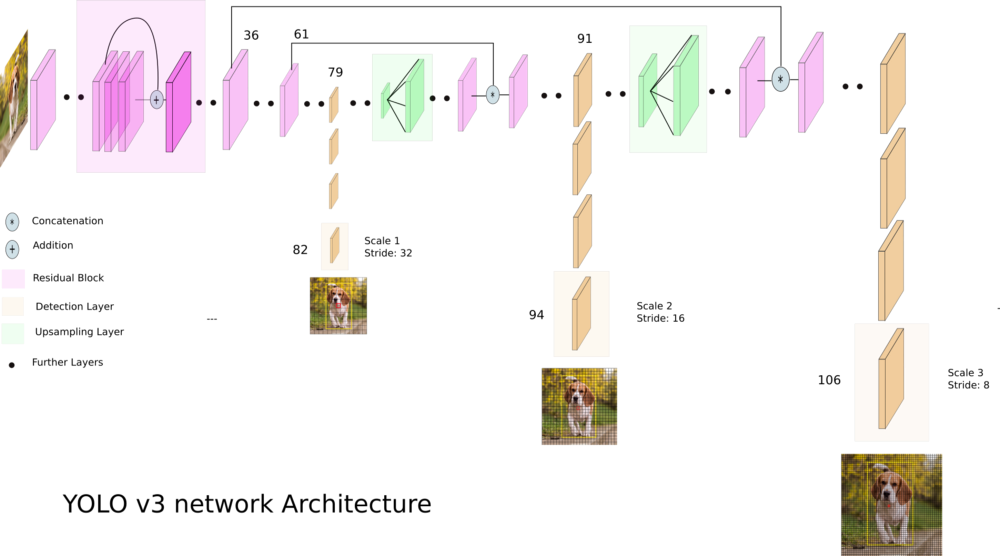
\includegraphics[width=0.85\linewidth]{figures/cnn/YOLOv3.png}}
    \caption{Architektura YOLOv3 se 106 vrstvami vytvářejícími predikce na třech různých rozlišeních (jmenovitě na vrstvách 82, 94 a~106).\footnotemark}
    \label{fig:YOLOv3}
\end{figure}

\footnotetext{Převzato z~\cite{yolov3_article}.}


%%%%%%%%%%%%%%%%%%%%%%%%%%%%%%%%%%%%%%%%%%%%%%%%%%%%%%%%%%%%%%%%%%%%%%%%%%%%%%%%%%%%%%%%%%%


\section{Single Shot Detector -- SSD}
\label{ssdTeorie}
Při studiu této problematiky jsem vycházel z~\cite{ssd}. Single shot detector (dále jen zkratka SSD), stejně jako YOLO, využívá pro detekci objektů jednu hlubokou neuronovou síť. Oba systémy SSD i~YOLO spadají do kategorie tzv. \emph{single-shot} detektorů. SSD je oproti ostatním metodám detekce objektů (R-CNN apod.) relativně jednoduché, protože odstraňuje krok návrhu kandidátních oblastí a~fáze převzorkování vlastností a~tedy dokáže zapouzdřit všechny výpočty do jediné neuronové sítě. Za pomoci detekce objektů množinou vrstev na \textbf{různých rozlišeních vstupního obrázku} lze dosáhnout relativně dobrých výsledků i~při nízkém rozlišení vstupní vrstvy, což mimo jiné také zvyšuje rychlost detekce a~snížení nároků na výpočetní zdroje. Systém SSD je založen na principu dopředné konvoluční neuronové sítě, která produkuje pevný počet ohraničujících boxů a~zároveň také pravděpodobnosti výskytu jednotlivých tříd v~daném boxu. Tento proces je následován tzv. \emph{non-maxima suppression} (potlačením ne-maximálních hodnot) pro odstranění duplikátních detekcí a~následným výstupem jednotlivých detekcí.

Vstupní vrstvy jsou založeny na běžném přístupu určeném pro klasifikaci objektů. Dále následují pomocné vrstvy sloužící pro vytvoření detekcí, skládající se z~aktivačních map o~různých rozměrech připojených za základní klasifikační část sítě. Tyto vrstvy slouží ke snížení rozměrů a~vytvoření predikcí na různým rozměrech vstupu, jak lze vidět na obrázku~\ref{fig:ssd}. Každá z~připojených aktivačních map může vytvářet pevný počet predikcí pomocí sady konvolučních filtrů a~to o~velikosti $3 \times 3 \times p$, kde $p$ označuje počet kanálů, udávající parametry možných detekcí. Tyto parametry udávají relativní odsazení detekovaného boxu od původního boxu a~pravděpodobnosti výskytu jednotlivých tříd. Pro každý z~$k$ boxů je predikováno $c$ pravděpodobností tříd a~$4$ hodnoty udávající odsazení k~původnímu boxu. Ve výsledku to pro obrázek velikosti $m \times n$ je $(c+4)mnk$ výstupních hodnot.

\begin{figure}[H]
    \centering
    \tmpframe{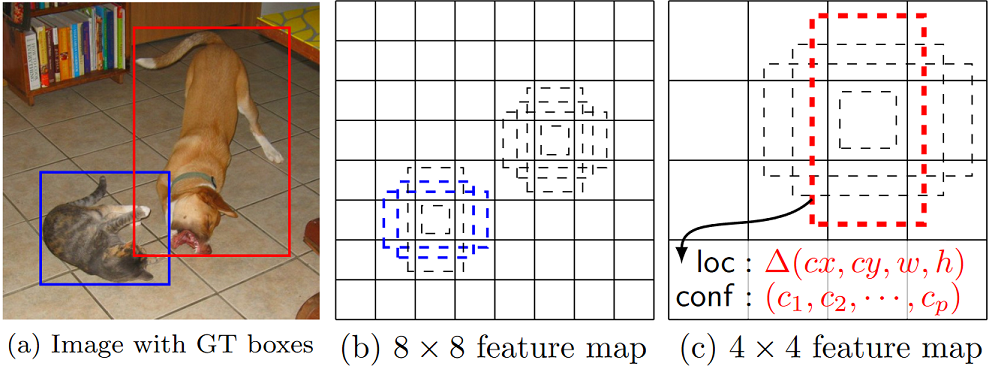
\includegraphics[width=0.85\linewidth]{figures/cnn/ssd.png}}
    \caption{Princip vytváření predikcí systémem SSD na různých rozměrech vstupního obrázku s~hodnotami odsazení vůči původnímu boxu a~skóre pravděpodobností jednotlivých tříd.\footnotemark}
    \label{fig:ssd}
\end{figure}

\footnotetext{Převzato z~\cite{ssd}.}

Pro výslednou detekci se aktivační mapy (různých rozměrů z~nižších i~vyšších vrstev) jedné konvoluční neuronové sítě kombinují dohromady pro dosažení vyšší jistoty (úspěšnosti) predikce.

%%%%%%%%%%%%%%%%%%%%%%%%%%%%%%%%%%%%%%%%%%%%%%%%%%%%%%%%%%%%%%%%%%%%%%%%%%%%%%%%%%%%%%%%%%%


\section{Region-based Convolutional neural network -- R-CNN}
\label{rcnnTeorie}
Při studiu této problematiky jsem vycházel z~\cite{rcnn,fast-rcnn,selective-search}. \emph{Region-based Convolutional neural network} (oblastní konvoluční neuronová síť, dále jen zkratka R-CNN) kombinuje návrh kandidátních oblastí, ve kterých se mohou nacházet objekty, s~klasifikací těchto oblastí založené na extrakci vlastností pomocí konvoluční sítě a~aplikování lineárního SVM. Obecný algoritmus zpracování, vizualizovaný na obrázku \ref{fig:rcnn}, je následující:

\begin{enumerate}
    \item Načtení vstupního snímku.
    \item Extrakce kolem 2000 oblastí ze vstupního obrázku pomocí selektivního vyhledávání.
    \item Extrakce vektoru vlastností z~jednotlivých oblastí pomocí komplexních konvolučních neuronových sítí.
    \item Klasifikace všech regionů pomocí sady tzv. \emph{class-specific} SVM.
\end{enumerate}

\begin{figure}[H]
    \centering
    \tmpframe{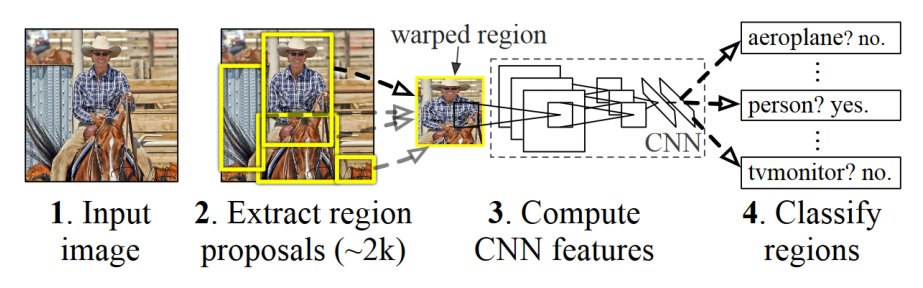
\includegraphics[width=0.85\linewidth]{figures/cnn/rcnn.eps}}
    \caption{Princip zpracování snímku pomocí R-CNN.\footnotemark}
    \label{fig:rcnn}
\end{figure}

\footnotetext{Převzato z~\cite{rcnn}.}

R-CNN využívá algoritmus selektivního hledání kandidátních oblastí představený v~prá-\\ci~\cite{selective-search}. Ta udává, že oblasti můžou obsahovat více informací než samotné pixely, proto by měly být při hledání upřednostňovány. Algoritmus je založen na nalezení několika počátečních oblastí a~následném iterativním shlukování oblastí (založeném na počítání podobnosti oblastí). Shlukování nejpodobnějších oblastí probíhá až do doby, kdy se celý snímek stane samostatnou oblastí. Protože algoritmus není invariantní vůči rozlišení vstupního snímku a~množství navržených oblastní závisí na jeho velikosti, musí se všem snímkům před provedením selektivního hledání změnit velikost na pevných $500\,\text{px}$.

Pro výpočet vstupního vektoru konvoluční sítě o~pevné délce z~navržené oblasti, nezávisle na jejím rozměru, se používá technika zvaná \emph{affine image warping}\footnotemark. Architektura konvoluční sítě má homogenní strukturu a~skládá se ze 13 konvolučních vrstev s~jádry o~velikosti $3 \times 3$. Mezi konvolučními vrstvami se nachází 5 maximalizačních sdružovacích vrstev a~architektura je zakončena třemi plně-propojenými vrstvami. Protože navržené oblasti mohou obsahovat jen část objektu, byl zvolen prah IoU $0.3$ -- pokud při validaci oblast překrývá \emph{ground-truth} o~méně než daný prah, je označena jako negativní. Při změně prahu na $0.5$ dojde k~poklesu mAP na datové sadě PASCAL VOC o~5 bodů \cite{rcnn}.

\footnotetext{\emph{Affine image warping} -- afinní obrazová deformace.}

Po získaní vlastností z~oblastí pomocí konvoluční sítě je použito jedno lineární SVM na každou třídu, které ohodnotí pravděpodobnost, zda vektor vlastností spadá do dané třídy. Poté je aplikováno potlačení ne-maximálních hodnot samostatně pro každou třídu, které ignoruje oblast, pokud má s~oblastí vyšší IoU, než je naučený prah.


\subsection*{Rychlejší verze -- Fast R-CNN}
\label{rcnnFast}
Ačkoli R-CNN dosahuje velmi dobré úspěšnosti detekce, doba vyhodnocení jednoho snímku trvá $\sim47$ sekund. Z~tohoto důvodu vznikly navazující verze Fast a~Faster (rychlá a~rychlejší) R-CNN. Zde je popsaná verze Fast R-CNN \cite{fast-rcnn}. Tato verze se snaží odstranit nevýhody R-CNN a~zároveň zvýšit rychlost a~úspěšnost detekce. Oproti R-CNN jsou během trénování upravovány všechny vrstvy, trénování je jedno-stupňové za použití více-úlohové ztrátové funkce a~extrahované vlastnosti už nejsou ukládány na disk.

Vstupem Fast R-CNN je vstupní snímek a~sada navržených oblastí, které jsou poté zpracovány, jak lze vidět na obrázku \ref{fig:fastrcnn}. Jako první je zpracován vstupní snímek pomocí několika konvolučních a~sdružovacích vrstev za účelem získání aktivační mapy. Poté jsou pro všechny navržené oblasti z~aktivačních map získány vektory vlastností pevné délky, které jsou posléze načteny do sady plně-propojených vrstev. Ty se poté větví do dvou posledních výstupních vrstev. Jedna slouží pro určení pravděpodobností jednotlivých tříd pomocí aktivační funkce softmax. Těchto tříd je celkem $K$ a~jedna specifická třída, která slouží k~odchycení veškerých detekcí pozadí. Druhá vrstva produkuje sadu 4 souřadnic predikovaných ohraničujících boxů pro každou z~$K$ tříd \cite{fast-rcnn}.

\begin{figure}[H]
    \centering
    \tmpframe{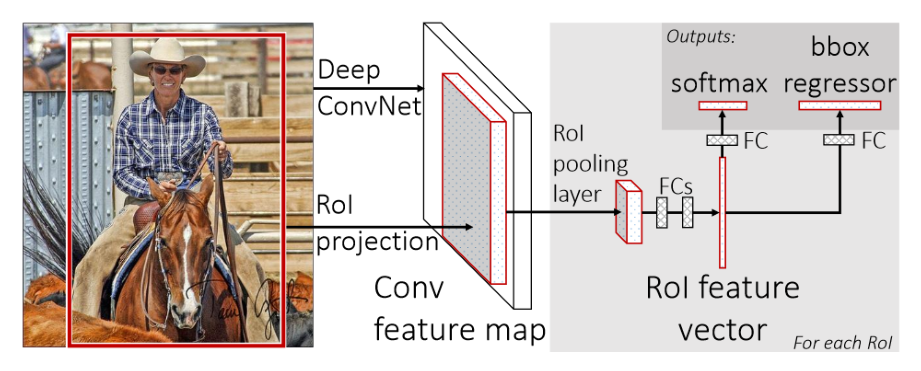
\includegraphics[width=0.85\linewidth]{figures/cnn/fastrcnn.eps}}
    \caption{Architektura systému Fast R-CNN.\footnotemark}
    \label{fig:fastrcnn}
\end{figure}

\footnotetext{Převzato z~\cite{fast-rcnn}.}

Výsledkem těchto úprav je, že:

\begin{itemize}
    \item Trénování Fast R-CNN je $9 \times$ rychlejší než trénování R-CNN.
    \item Detekce jednoho snímku provádí Fast R-CNN $213 \times$ rychleji.
    \item Na datové sadě PASCAL VOC 2012 dosahuje Fast R-CNN lepší úspěšnosti $66\,\%$ mAP (oproti $62\,\%$ R-CNN).
\end{itemize}


\chapter{Návrh systému pro detekci dopravního značení}
\label{navrhDetektoru}
Tato kapitola se zabývá porovnáním jednotlivých technik pro detekci a~klasifikaci značek popsaných v~kapitolách \ref{detekceZnacek} a~\ref{detekceKonv}, návrhem systému pro detekci dopravního značení, a~také porovnáním datových sad a~neuronových sítí, které lze použít k~trénování a~testování.

%%%%%%%%%%%%%%%%%%%%%%%%%%%%%%%%%%%%%%%%%%%%%%%%%%%%%%%%%%%%%%%%%%%%%%%%%%%%%%%%%%%%%%%%%%%

\section{Datové sady dopravního značení}
\label{datoveSady}
Datové sady jsou neodmyslitelnou součástí strojového učení. Dostatek datových sad je jedním z~důvodů, proč se neuronové sítě staly v~dnešní době tak populárními. Datových sad dopravních značek existuje spousta, avšak většina z~nich obsahuje pouze vyřezané dopravní značky z~celých snímků, na kterých se běžně trénují klasifikátory (tedy systémy, které slouží pouze k~rozhodnutí o~třídě značky, nikoli k~detekci a~lokalizaci v~rámci celého snímku). Běžná velikost snímků v~takovýchto sadách bývá velmi malá, například $64 \times 64$ pixelů. Jak je popsáno v~sekci \ref{yoloTeorie}, systém YOLO použitý v~této práci pro detekci se trénuje na tzv. celých (nebo také plných) snímcích. Dokáže se z~nich naučit jak celkový kontext, tak i~relativní velikost detekovaných značek. Proto bylo potřeba najít takovou datovou sadu, která bude obsahovat celé snímky.

Podařilo se najít čtyři takové datové sady dopravních značek: Německou (GTSD) \cite{gtsd}, Belgickou (BTSD) \cite{btsd}, Ruskou (RTSD) \cite{rtsd} a~Americkou, kde však používají naprosto rozdílnou normu dopravního značení, a~proto byla v~rámci této práce nepoužitelná. Počáteční písmeno těchto datových sad běžně slouží k~jejich identifikaci (název státu, kde byly snímky pořízeny) a~končí písmenem ``D'', které je zkratkou pro anglické \emph{detection} a~běžně značí, že se jedná o~datovou sadu s~celými snímky používanými pro detekci. Stejně tak ``C'' jako \emph{classification}. V~tabulce \ref{tabulkaDatasety} lze najít velikost jednotlivých sad, dále pak počet tříd a~značek v~nich obsažených.

\begin{table}[H]
	\vskip6pt
	\centering
    \begin{tabular}{ l | c | c | c }
        Datová sada & Počet snímků & Počet tříd & Počet značek \\
        \toprule
        GTSD \cite{gtsd} & 900 & 43 & 1213 \\
        BTSD \cite{btsd} & 25630 & 108 & 13444 \\
        RTSD \cite{rtsd} & 179138 & 156 & 104358 \\
    \end{tabular}
    \caption{Tabulka velikostí, počtu tříd a~značek jednotlivých datových sad značek.}
    \vskip6pt
    \label{tabulkaDatasety}
\end{table}

Na obrázku \ref{fig:datasety} lze vidět ukázku snímků z~jednotlivých datových sad. Jak lze vidět v~tabulce \ref{tabulkaDatasety}, velikost jednotlivých datových sad se liší. Stejně tak se liší kvalita, velikosti a~anotace snímků.

\begin{figure}[H]
    \centering
    \tmpframe{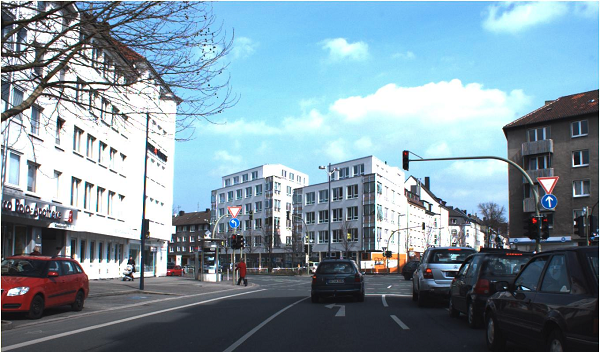
\includegraphics[width=0.33\linewidth]{figures/datasety/gtsd.png}}\hfill
    \tmpframe{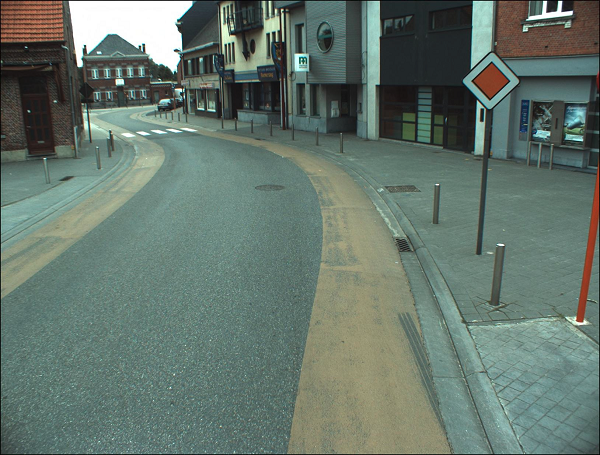
\includegraphics[width=0.33\linewidth]{figures/datasety/btsd.png}}\hfill
    \tmpframe{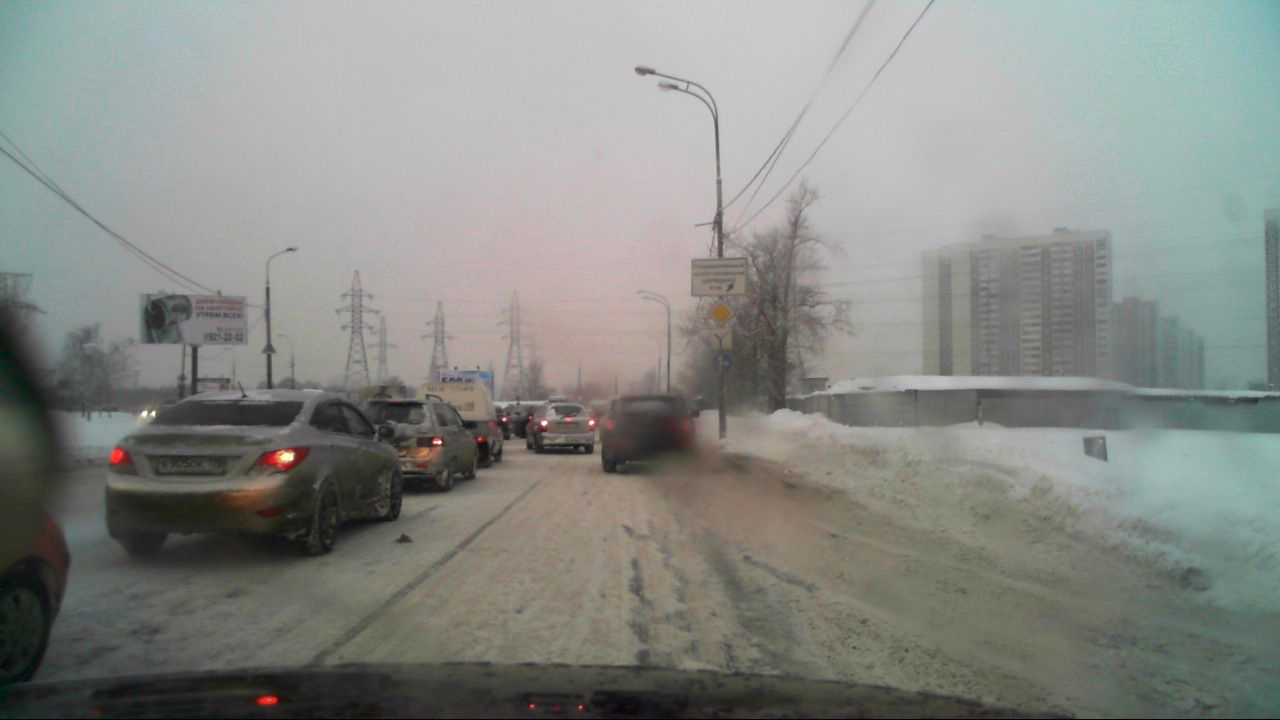
\includegraphics[width=0.33\linewidth]{figures/datasety/rtsd.png}}
    \caption{Ukázka snímků datových sad (\textbf{zleva}) GTSD, BTSD a~RTSD.}
    \label{fig:datasety}
\end{figure}

Nejvyšší kvalitu má Německá datová sada, tedy GTSD, avšak nevýhoda této sady je velmi malý počet značek na třídu -- v~průměru to je cca. 28, a~to pro natrénování a zároveň vyhodnocení kvalitního detektoru nestačí. Ruská datová sada má naopak značek na třídu dost, ale kvalita těchto značek a~snímků obecně je velmi špatná. Značky jsou malé a~rozmazané. Jako dostatečná se tedy jeví Belgická sada, která má poměrně dost snímků i~dobrou kvalitu, ale nevýhodou této sady je, že téměř dvě třetiny datové sady je pouze tzv. \emph{negativní datová sada} (neobsahující žádné značky). I přes to ale byla tato sada vybrána jako hlavní pro trénování i testování.


%%%%%%%%%%%%%%%%%%%%%%%%%%%%%%%%%%%%%%%%%%%%%%%%%%%%%%%%%%%%%%%%%%%%%%%%%%%%%%%%%%%%%%%%%%%


\section{Návrh generátoru syntetických dat}
Z~důvodu nedostatku datových sad dopravních značek s~plnými snímky, a~také za účelem porovnání detektoru trénovaného na reálných a~syntetických datech jsem se rozhodl v~rámci této práce vytvořit generátor syntetických datových sad. Cílem bylo iterativně zlepšovat generátor, aby výsledná data co nejvíce odpovídala reálným snímkům a~zlepšování výsledků, aby se kvalita detektoru trénovaného na syntetických datech vyrovnala, či dokonce překonala kvalitu detektoru trénovaného na reálných datech. Testování obou detektorů probíhalo na reálných snímcích Belgické sady. Aby se syntetická data co nejvíce podobala reálným snímkům, je potřeba dosáhnout velké variability snímků simulující různé světelné podmínky, přírodní vlivy, natočení, vandalismus, apod. To následně umožňuje hluboké konvoluční síti se naučit dostatek vlastností a~dokázat správně generalizovat na reálných snímcích. Z důvodu, že se zvolená metoda YOLO učí i~celkový kontext ve kterém se objekty nachází, byly pro generování využity jako pozadí snímky zachycené z~jedoucího vozidla (převážně v~městské zástavbě), neobsahující žádné značky. Značky, které by nebyly anotovány a negativně by ovlivňovaly proces trénování.

Alternativním způsobem pro získání kvalitní dostatečně velké anotované datové sady, bez nutnosti anotace každého snímku jednotlivě, by bylo využití existujícího detektoru značek (pokud možno toho s~nejvyšší úspěšností) a~jeho aplikování na ne-anotovanou datovou sadu. Poté by stačilo výsledky projít a~případně upravit nevalidní detekce, což by zabralo podstatně méně času, než anotovat celou datovou sadu ručně. Protože částečným cílem práce je i~porovnání modelů trénovaných na reálných a~syntetických datech, rozhodl jsem se tento způsob nevyužít a~soustředit se na tvorbu syntetické datové sady.


%%%%%%%%%%%%%%%%%%%%%%%%%%%%%%%%%%%%%%%%%%%%%%%%%%%%%%%%%%%%%%%%%%%%%%%%%%%%%%%%%%%%%%%%%%%


\section{Porovnání a~výběr metod pro detekci a~klasifikaci}
\label{navrhDetekce}
Tato práce si dává za cíl použití \textbf{moderních technik pro detekci}, a~proto se do užšího výběru dostaly pouze metody jako SSD, YOLO, Fast(er) R-CNN a~RetinaNet. V~tabulce~\ref{tab:porovnaniMetody} lze vidět komplexní porovnání úspěšností těchto metod na datové sadě COCO. Tabulka zobrazuje úspěšnost AP v~závislosti na různých prazích IoU a~různých velikostech detekovaných objektů (\emph{small}, \emph{medium} a~\emph{large}, tzn. malé, střední a velké). Tabulka je rozdělena na dvě části podle počtu kroků vykonávaných systémem při detekci. Protože při detekci je důležitá také rychlost, je na obrázku \ref{fig:porovnaniDetektoru} graficky znázorněno porovnání metod podle času potřebného pro vyhodnocení jednoho snímku v~závislosti na úspěšnosti.

\begin{table}[H]
	\vskip6pt
	\centering
    \begin{tabular}{ l | c | c c c | c c c }
        & Backbone & AP & AP_{50} & AP_{75} & AP_S & AP_M & AP_L \\
        \toprule
        \emph{Two-stage methods} & & & & & & & &
        Faster R-CNN+++ & ResNet-101-C4 & 34.9 & 55.7 & 37.4 & 15.6 & 38.7 & 50.9 \\
        Faster R-CNN & ResNet-101-FPN & 36.2 & 59.1 & 39.0 & 18.2 & 39.0 & 48.2 \\
        w FPN & & & & & & & \\
        Faster R-CNN & Inception-ResNet-v2 & 34.7 & 55.5 & 36.7 & 13.5 & 38.1 & 52.0 \\
        by G-RMI & & & & & & & \\
        Faster R-CNN & Inception-ResNet-v2 & 36.8 & 57.7 & 39.2 & 16.2 & 39.8 & \textbf{52.1} \\
        w TDM & TDM & & & & & & \\
        \hline
        \emph{One-stage methods} & & & & & & & &
        YOLOv2 & DarkNet-19 & 21.6 & 44.0 & 19.2 & 5.0 & 22.4 & 35.5 \\
        SSD513 & ResNet-101-SSD & 31.2 & 50.4 & 33.3 & 10.2 & 34.5 & 49.8 \\
        DSSD513 & ResNet-101-DSSD & 33.2 & 53.3 & 35.2 & 13.0 & 35.4 & 51.1 \\
        RetinaNet & ResNet-101-FPN & 39.1 & 59.1 & 42.3 & 21.8 & 42.7 & 50.2 \\
        RetinaNet & ResNeXt-101-FPN & \textbf{40.8} & \textbf{61.1} & \textbf{44.1} & \textbf{24.1} & \textbf{44.2} & 51.2 \\
        YOLOv3 $608 \times 608$ & Darknet-53 & 33.0 & 57.9 & 34.4 & 18.3 & 35.4 & 41.9 \\
    \end{tabular}
    \caption{Porovnání detekčních metod na různých metrikách~\cite{yolov3}.} 
    \vskip6pt
    \label{tab:porovnaniMetody}
\end{table}

Jak lze z~tabulky vyčíst, rozdíl mezi SSD a~YOLOv3 v~rámci úspěšnosti při použití moderní metriky AP, počítané na 10 různých prazích IoU, není velký a~oba tyto systémy předčil model RetinaNet. Při použití tradiční metriky $AP_{50}$, počítané pouze na $\text{IoU} = 0.5$ má YOLOv3 velmi dobrou úspěšnost srovnatelnou s~RetinaNet a~podstatně lepší úspěšnost než obě verze SSD. Se zvyšujícím se prahem IoU značně klesá úspěšnost metod YOLOv3 a~SSD, což indikuje nedokonalou lokalizaci objektů (predikované boxy neodpovídají přesně \emph{ground-truth}, tedy skutečné pozici objektů).

Protože u~SSD slouží k~detekci pouze několik počátečních vrstev, je úspěšnost detekce malých objektů poměrně nízká. V~minulosti mělo s~detekcí malých objektů velké problémy i~YOLO, ale třetí verze provádějící detekci na třech různých rozlišeních značně zlepšila jejich detekci, ale stále je podstatně nižší než u~RetinaNet.

\begin{figure}[H]
    \centering
    \tmpframe{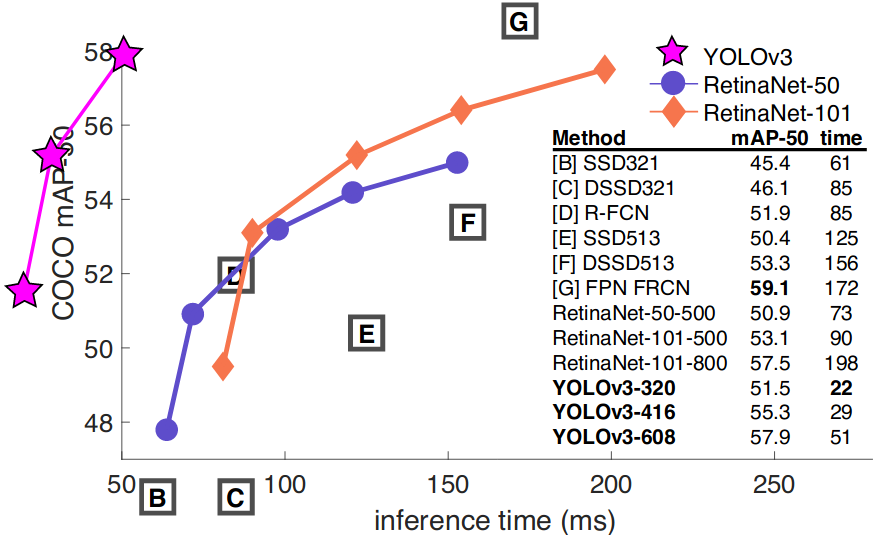
\includegraphics[width=0.85\linewidth]{figures/navrh/porovnaniDetektoru.png}}
    \caption{Porovnání detekčních systémů v~poměru úspěšnosti a~rychlosti vyhodnocení detekce na GPU Titan X.\footnotemark}
    \label{fig:porovnaniDetektoru}
\end{figure}

\footnotetext{Převzato z~\cite{yolov3}.}

YOLOv3 je jednoznačně nejrychlejší metodou ze všech uvedených a~i~přesto dosahuje velmi dobré úspěšnosti detekce. Odlehčená verze dokonce dosahuje dokonce rychlosti až 150 snímků za sekundu výměnou za několik bodů mAP. Při použití běžné grafické karty (oproti Titan X, na níž jsou uvedené rychlosti získány) výrazně klesne rychlost trénování a~zejména detekce, a~proto jsem se rozhodl použít systém Tiny YOLOv3, což je již zmíněná odlehčená verze systému YOLOv3, se kterou by bylo možné dosáhnout zpracování v~reálném čase i~na běžné grafické kartě a~přitom dosáhnout dobré úspěšnosti detekce.


%%%%%%%%%%%%%%%%%%%%%%%%%%%%%%%%%%%%%%%%%%%%%%%%%%%%%%%%%%%%%%%%%%%%%%%%%%%%%%%%%%%%%%%%%%%


\section{Neuronová síť Darknet}
\label{navrhDarknet}
Darknet \cite{darknet} je \emph{open-source} (česky otevřený software) aplikační rámec neuronové sítě napsané v~programovacím jazyce \texttt{C} a~\texttt{CUDA}\footnotemark. Je možné s~ním provádět výpočty jak na CPU (procesoru), tak na GPU (grafické kartě). \emph{Darknet} je možné používat jak na operačním systému Linux, tak i~upravenou verzi na systému Windows.

\begin{table}[H]
	\vskip6pt
	\centering
    \begin{tabular}{ l | c c c c c }
        Backbone & Top-1 & Top-5 & Bn Ops & BFLOPS/s & FPS \\
        \toprule
        Darknet-19 & 74.1 & 91.8 & 7.29 & 1246 & \textbf{171} \\
        ResNet-101 & 77.1 & 93.7 & 19.7 & 1039 & 53 \\
        ResNet-152 & \textbf{77.6} & \textbf{93.8} & 29.4 & 1090 & 37 \\
        Darknet-53 & 77.2 & \textbf{93.8} & 18.7 & \textbf{1457} & 78 \\
    \end{tabular}
    \caption{Porovnání neuronových sítí: Přesnost, počet bilionů operací bez i~s~plovoucí řádovou čárkou a~počet snímků za sekundu~\cite{yolov3}.} 
    \vskip6pt
    \label{tab:porovnaniBackbones}
\end{table}

 Kvůli parametrům neuronové sítě Darknet-53 jsem se rozhodl ji použít v této práci.

\footnotetext{CUDA -- \emph{Compute Unified Device Architecture}.}


\chapter{Implementace navrženého detektoru}
\label{implementaceDetektoru}
V~této kapitole je popsána implementace generátoru syntetických datových sad vytvořeného v~rámci této práce. Dále je zde popsán proces vytváření detektoru dopravních značek, jeho trénovaní, vyhodnocení a~iterativního zlepšování úspěšnosti.


%%%%%%%%%%%%%%%%%%%%%%%%%%%%%%%%%%%%%%%%%%%%%%%%%%%%%%%%%%%%%%%%%%%%%%%%%%%%%%%%%%%%%%%%%%%


\section{Generátor syntetických datových sad}
\label{syntDataset}
Generování syntetických datových sad pro trénování hlubokých neuronových sítí se stává čím dál populárnější technikou, která usnadňuje proces trénovaní o~nutnost anotovat datovou sadu (či rozšíření existující datové sady) a~zároveň umožňuje dosažení dobré úspěšnosti detekce/klasifikace. Avšak problém je dokázat generovat datovou sadu tak, aby model na ní trénovaný dokázal správně generalizovat na reálných snímcích, což je čím dál častěji předmětem výzkumu a~bude popsáno i~v~této práci.

Pro generování se nabízí hned několik způsobů. Aplikační rámce jako např. PyTorch či TensorFlow obsahují zabudované \uv{generátory}, které lze využít pro rozšíření již existující datové sady. Ty fungují na principu modifikace jednotlivých snímků datové sady (např. otočení snímku kolem osy \emph{y}, změna světelných podmínek, apod.) a~jejich následné připojení k~datové sadě. Další způsob využívaný zejména pro komplexní objekty, jako je například tvář člověka, je vymodelování objektu (např. v~programu \emph{Blender}) a~poté pomocí skriptu \uv{nafocení} tohoto objektu z~různých uhlů a~za různých světelných podmínek. Pro generování plných snímků, které jsou pro trénování neuronové sítě YOLO potřeba, lze využít techniku umisťování těchto objektů do snímků pozadí a~modifikaci jejich vzhledu za účelem dosažení větší variability vzniklé datové sady. Poslední zmíněnou technikou je GAN\footnotemark. Tato technika, jak již jméno napovídá, je založena na \uv{zápasení} dvou neuronových sítí a~slouží mimo jiné pro generování syntetických snímků. Je to ovšem metoda učení bez učitele, a~proto se nedá použít pro generování objektů do plných snímků.

\footnotetext{GAN -- \emph{Generative adversarial network}.}

Systém YOLO je trénovaný na plných snímcích, a~proto jak bylo navrženo, byl v~této práci využit způsob umisťování dopravních značek do plných snímků pozadí. Dále byla získána sada snímků z~palubní kamery a~veškeré snímky obsahující dopravní značky byly odstraněny, protože by negativně ovlivňovaly proces trénovaní.

\subsection*{Efekty aplikované na značky}
\label{syntDatasetEfekty}
Aby bylo dosaženo větší variability datové sady a~konvoluční neuronová síť se byla schopna naučit co nejvíce vlastností dopravních značek, bylo před samotným vložením značky do pozadí provedeno několik operací upravující vzhled značky. Seznam operací, které se s~určitou pravděpodobností aplikují na vyřezané dopravní značky, je následující:

\begin{itemize}
    \item \textbf{Gamma korekce} -- Slouží k~simulaci různých světelných podmínek. Pravděpodobnost aplikace tohoto efektu je $15\,\%$.
    \item \textbf{Úprava jasu} -- Slouží k~simulaci různých světelných podmínek. Pravděpodobnost aplikace tohoto efektu je $15\,\%$.
    \item \textbf{Úprava jasu podle pozadí} -- Slouží k~získání průměrného osvětlení v~místě, kam bude dopravní značka umístěna a~následné úpravě jasu značky podle získané hodnoty. Lze nahradit za předchozí efekt.
    \item \textbf{\emph{Salt and pepper} šum} -- Slouží k~simulaci poškození značky. Pravděpodobnost aplikace tohoto efektu je $5\,\%$.
    \item \textbf{Gaussovský šum} -- Slouží k~simulaci poškození značky. Pravděpodobnost aplikace tohoto efektu je $5\,\%$.
    \item \textbf{Překrytí části značky} -- Simuluje běžně se vyskytující překrytí značky. Pravděpodobnost aplikace tohoto efektu je $5\,\%$.
    \item \textbf{Gradient osvětlení} -- Simuluje reálné osvětlení značek. Pravděpodobnost aplikace tohoto efektu je $15\,\%$.
    \item \textbf{Rotace v~ose Z} -- Simuluje záběr z~různých úhlů. Pravděpodobnost aplikace tohoto efektu je $25\,\%$.
    \item \textbf{Rotace v~ose Y} -- Simuluje záběr z~různých úhlů. Pravděpodobnost aplikace tohoto efektu je $25\,\%$.
    \item \textbf{Rozmanání značky} -- Simuluje vyšší rychlost vozidla či nižší kvalitu kamery. Pravděpodobnost aplikace tohoto efektu je $5\,\%$.
    \item \textbf{Úprava barvy (HSV)} -- Simuluje značky různých Evropských norem (viz obrázek~\ref{kolazStopky}). Pravděpodobnost aplikace tohoto efektu je $10\,\%$.
    \item \textbf{Změna velikosti značky} -- Simuluje různé vzdálenosti značky od kamery. Pravděpodobnost aplikace tohoto efektu je $90\,\%$.
\end{itemize}

Naopak techniky, které úspěšnost nezvýšily, či dokonce snížily jsou následující:

\begin{itemize}
    \item Rotace značky kolem osy \emph{y}
    \item Přidání luminiscenčního podkladu značek
    \item Přidání ocelové konstrukce značek
    \item Výběr pozic, kam značku umístit a~následná úprava velikosti podle umístění
\end{itemize}

Z~důvodu, že se dopravní značky nachází většinou po stranách silnice, bylo provedeno několik pokusů s~umisťováním značek pouze na okraje, a~to tak že čím blíže byly středu, tím menší velikosti nabývaly (simulace reálného prostředí). Tyto pokusy však neprokázaly zvýšení úspěšnosti. Luminiscenční podklad i~ocelová konstrukce měly za úkol přidat přirozený kontext, ve kterém se značky nachází. Tyto přidané objekty ovšem výrazně snižovaly úspěšnost detekce. Jedna z~vlastností mnoha značek je, že jsou osově souměrné, a~proto byla vyzkoušena také rotace značek kolem osy \emph{y} (kromě značek obsahující šipky vlevo/vpravo apod.), ale ke zlepšení úspěšnosti to nevedlo.

\subsection*{Způsob generování s~transparentními značkami}
\label{syntDatasetTransparent}
Tato technika je založena na principu umisťování transparentních značek (obsahující alfa-kanál) do snímků pozadí. Výhodou tohoto přístupu je, že kolem značky nevzniká výrazná přestupná hrana, jako je tomu u~druhého způsobu používající vyřezané značky.

\begin{figure}[H]
    \centering
    \tmpframe{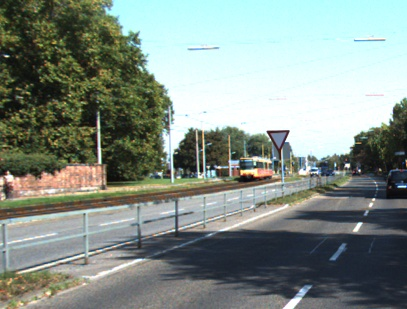
\includegraphics[width=0.495\linewidth]{figures/implementace/giveway_transparent.png}}\hfill
    \tmpframe{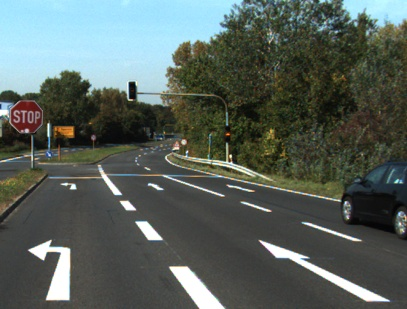
\includegraphics[width=0.495\linewidth]{figures/implementace/stop_transparent.png}}\\
    \tmpframe{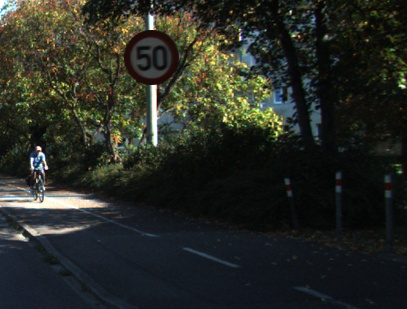
\includegraphics[width=0.495\linewidth]{figures/implementace/synt_50.png}}\hfill
    \tmpframe{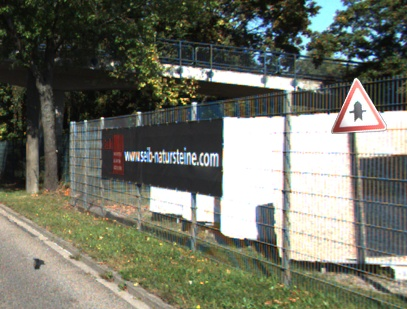
\includegraphics[width=0.495\linewidth]{figures/implementace/synt_junction.png}}
    \caption{Příklad vygenerovaných dat za pomoci transparentních značek. Značkám bylo před vložením do snímku pozadí upraveno osvětlení, velikost a~natočení.}
    \label{fig:datasetCropped}
\end{figure}

Naopak nevýhodou tohoto přístupu je, že aby bylo dosaženo jisté variability takto vygenerované datové sady, bylo by potřeba velké množství značek vyřezaných z~reálných snímků. Tento problém se dá řešit pomocí již zmíněných efektů aplikovaných na dopravní značky popsaných v~sekci \ref{syntDatasetEfekty} a~vizualizovaných na obrázku \ref{fig:stopImplementace}.

\begin{figure}[H]
    \centering
    \tmpframe{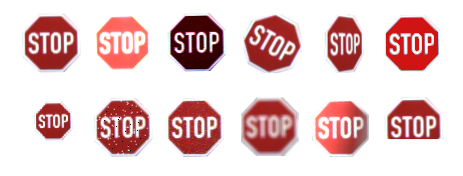
\includegraphics[width=0.99\linewidth]{figures/implementace/znacky.png}}
    \caption{Příklad aplikace všech efektů modifikujících vzhled dopravních značek na jedné značce typu \emph{stop}. Originál vlevo nahoře.}
    \label{fig:stopImplementace}
\end{figure}

Pravděpodobnost aplikace efektu je dána pravděpodobností s~rovnoměrných rozložením, takže se běžně stává, že se aplikuje více efektů na jednu značku (například natočení, změna jasu i~přidání šumu). Každý efekt používá jiné hodnoty, například natočení značky se udává ve stupních. Z~daného, předem definovaného, rozsahu aplikovaných hodnot se pseudonáhodně vybere hodnota při každé aplikaci efektu. Kdyby se při každé aplikaci efektu používaly stejné hodnoty, vzhled značek by se začal brzy opakovat.

Pravděpodobnost aplikace efektu i~rozsah aplikovaných hodnot byly pečlivě vybírány a~upravovány jak pomocí experimentů, tak inspirací vzhledu značek z reálného světa. Například vizuálně poškozené značky se příliš často nevyskytují, proto byla pro přidání šumu zvolena poměrně nízká pravděpodobnost. Naopak různé světelné podmínky či natočení značek jsou běžně se vyskytující jevy, proto jim byla přiřazena poměrně vysoká pravděpodobnost aplikace.

Při implementaci jednotlivých efektů byla vždy prováděna kontrola realističnosti vzhledu vygenerovaných značek. Tzn. zda vygenerované značky vypadají jako by pocházely z~reálného světa. Dosažení opravdu reálného vzhledu je velmi problematické a~vyžadovalo by složitou 3D analýzu jak značky, tak pozadí, kam se značka umisťuje. Ani při dosažení realistického vzhledu (pro člověka) není jisté, zda se dokáže neuronová síť naučit potřebné vlastnosti a~dokáže poté správně generalizovat na reálných snímcích. Lidské oko je totiž více citlivé na jiné faktory, než počítač.

\subsection*{Způsob generování s~ořezanými značkami}
\label{syntDatasetOrezane}
Tento způsob je založen na použití reálných snímků vyřezaných dopravních značek určených pro trénování klasifikátorů. Těchto značek je velké množství, ale nevýhodou je, že po vložení do snímku pozadí kolem těchto značek vzniká výrazná přestupná hrana, jak lze vidět na obrázku \ref{fig:datasetCropped} (vlevo), která negativně ovlivňuje proces trénování. Řešením je použití tzv. \emph{Poisson blending}, které kombinuje gradienty a~intenzity barev obou obrázků a~ve výsledku to vypadá tak, že objekt do daného kontextu patří. Nevýhodou je, že algoritmus \emph{Poisson blending} začíná počítat pouze od hraničních bodů, kam se objekt umisťuje, a~proto pokud jsou tyto hraniční body příliš světlé, sníží se i~intenzita barev vkládané značky a~ve výsledku není téměř vidět. Podobně tomu je pokud jsou hraniční body příliš tmavé, až černé \cite{poissonEditing}. Příklad výsledku vložení pomocí techniky \emph{Poisson blending} lze vidět na obrázku \ref{fig:datasetCropped} (vpravo). Použité vyřezané značky pochází z~Německé datové sady, protože použití značek vyřezaných z~Belgické datové sady, na které se později provádělo vyhodnocení by mohlo zkreslit výsledky.

\begin{figure}[H]
    \centering
    \tmpframe{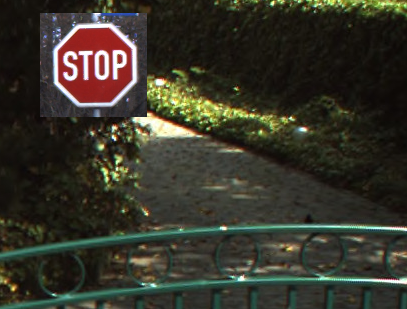
\includegraphics[width=0.49\linewidth]{figures/implementace/stop_cropped.png}}\hfill
    \tmpframe{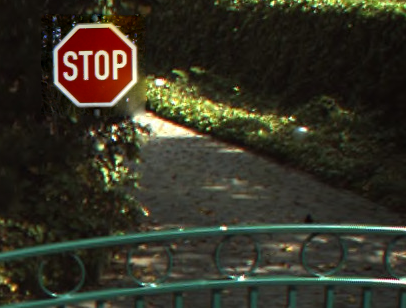
\includegraphics[width=0.49\linewidth]{figures/implementace/stop_poisson.png}}
    \caption{Porovnání vložení ořezané dopravní značky do pozadí bez použití (\textbf{vlevo}) a~s~použitím (\textbf{vpravo}) techniky \emph{Poisson blending}.}
    \label{fig:datasetCropped}
\end{figure}


\subsection*{Množství generovaných dat}
Pro trénování na syntetických datech bylo potřeba zjistit optimální počet generovaných značek na třídu. V~tabulce \ref{tab:pocetSnimkuUspesnost} lze vidět závislost počtu syntetických snímků na výsledné úspěšnosti. Jak lze z~tabulky vyčíst, mezi $200$, $500$ a~$1000$ snímky se vyskytují velké skoky v~úspěšnosti, zatímco mezi $1000$ a~$2000$ se úspěšnost již téměř nezvýšila, zato se razantně prodloužila doba trénování. Jako optimální počet pro budoucí trénování na syntetických datech tedy vyšlo $1000$ značek na třídu.

\begin{table}[h]
	\vskip6pt
	\caption{Závislost úspěšnosti YOLOv3-608 na množství syntetických snímků na třídu.}
	\centering
	\begin{tabular}{cc}
		\toprule
		Počet snímků & Úspěšnost v~mAP\\
		\midrule
		$200$  & $63.2\,\%$ \\
		$500$  & $77.9\,\%$ \\
		$\textbf{1000}$ & $86.3\,\%$ \\
		$2000$ & $\textbf{87.6}\,\%$ \\
		\bottomrule
	\end{tabular}
	\label{tab:pocetSnimkuUspesnost}
\end{table}

%%%%%%%%%%%%%%%%%%%%%%%%%%%%%%%%%%%%%%%%%%%%%%%%%%%%%%%%%%%%%%%%%%%%%%%%%%%%%%%%%%%%%%%%%%%

\section{Konfigurace neuronové sítě při trénovaní a~testování}
\label{cnnKonfigurace}
Pro konfiguraci neuronové sítě se používá konfigurační soubor, \texttt{yolo-train.cfg}, při jehož studiu a~popisu jsem vycházel z~\cite{darknet_config, darknet_anchors}. Nejdůležitější parametry, které lze v~rámci konfiguračního souboru nastavit a~se kterými bylo v~rámci této práce experimentováno jsou následující:

\begin{itemize}
    \item \textbf{anchors} -- Výstupní hodnoty neuronové sítě YOLO neudávají přímo výšku a~šířku ohraničujícího boxu, ale udávají pouze \emph{offset} vůči před-definovaným \uv{kotvám} (anglicky \textbf{\emph{anchors}}) s~nejvhodnější velikostí. Tyto kotvy se vyskytují ve vrstvách \texttt{[yolo]} a~jsou definovány následovně: \texttt{anchors = 4,7, 7,15, 13,25,   25,42, 41,67,\\ 75,94, 91,162, 158,205, 250,332}.
    \item \textbf{mask} -- Každá \texttt{[yolo]} vrstva potřebuje vědět o~všech kotvách, ale jen některé z~nich může použít. Proto se do těchto vrstev zavedl seznam \emph{mask}, ve kterém se udají indexy kotev, které smí daná vrstva použít. Pro použití pouze prvních třech kotev lze použít \texttt{mask = 0,1,2}.
    \item \textbf{filters} -- Udává počet konvolučních jader v~dané vrstvě. Nejvhodnější počet filtrů je podle autorů \texttt{filters = (num\_classes + 5) * 3}. Hodnota 5 označuje počet predikovaných hodnot pro jeden ohraničující box (x, y, výška, šířka a~skóre \emph{objectness}) a~3 v~tomto případě označuje počet kotev.
    \item \textbf{activation} -- Určuje aktivační funkci vrstvy. Může být např. \emph{ReLu}, \emph{sigmoid}, \emph{tanh}, \emph{linear}, \emph{leaky}, apod.
    \item \textbf{random} -- Pokud se rovná jedné, daná vrstva mění velikost vstupního snímku vždy po několika dávkách na různé velikosti.
    \item \textbf{angle} -- Otočení vstupního snímku o~uvedený počet stupňů.
    \item \textbf{batch} -- Dávka, tedy množství snímků k~dopředné propagaci skrze neuronovou síť sloužící k~výpočtu gradientu, který se poté používá k~úpravě vah pomocí zpětné propagace.
    \item \textbf{subdivisions} -- Dávka je rozdělena do tohoto množství bloků. Autoři neuronové sítě Darknet uvádí, že jednotlivé bloky \emph{subdivisions} jsou počítány na GPU paralelně, ovšem trénování při \texttt{subdivisions=16} bylo pomalejší, než když byl tento parametr roven čtyřem či osmi.
    \item \textbf{flip} -- Pokud je nastaven na $1$, jsou snímky po několika dávkách otočeny. Podle autorů zvyšuje použití této funkce úspěšnost, ale protože je potřeba rozlišit značky s~šipkami vlevo/vpravo, nebylo možné jej v~rámci této práce použít.
    \item \textbf{step} -- Určuje po kolika dávkách se má upravit učící faktor.
\end{itemize}

Dále je potřeba nastavit v souboru \texttt{obj.data} počet tříd, cesty k trénovací a validační datové sadě, soubor se jmény jednotlivých tříd (\texttt{obj.names}) a cestu, kam se budou ukládat váhy modelu.

%%%%%%%%%%%%%%%%%%%%%%%%%%%%%%%%%%%%%%%%%%%%%%%%%%%%%%%%%%%%%%%%%%%%%%%%%%%%%%%%%%%%%%%%%%%

\section{Trénování neuronové sítě}
Trénování neuronové sítě je zpravidla proces velmi náročný na výpočetní prostředky (záleží na konfiguraci parametrů sítě) a~není jej tedy vhodné (mnohdy ani možné) provádět na osobním počítači. Tato podkapitola se zabývá všemi aspekty, které bylo potřeba splnit k~úspěšnému natrénování sítě včetně experimentů.

\subsection*{Sdílený cluster}
Proces trénování hluboké konvoluční neuronové sítě je velmi náročný na výpočetní prostředky. To je jeden z~důvodů, proč nelze komplexní neuronové sítě s~velkým počtem vstupů a~vrstev trénovat na běžných osobních počítačích a~bylo tedy potřeba najít výkonný sdílený cluster, na kterém bude možné výpočty provádět. Tyto služby, kterých jsem po značnou část práce využíval, poskytuje pro akademickou obec zdarma virtuální organizace MetaCentrum~\cite{metacentrum}.

MetaCentrum funguje na principu vytváření úloh pomocí plánovacího systému PBS\footnotemark. Na začátku je nutné vytvořit dávkový skript, který obsahuje posloupnost instrukcí, jež se mají na sdíleném clusteru v rámci úlohy vykonat. Poté je potřeba úlohu naplánovat, tedy zařadit do fronty, kde bude čekat na spuštění (až úloha přijde na řadu a bude dostatek požadovaných zdrojů). V~rámci plánování úlohy je možné specifikovat, jaké zdroje úloha potřebuje. Doba strávená ve frontě je úměrná množství požadovaných výpočetních prostředků.

Obecné parametry, které se běžně specifikují, jsou například počet procesorů, grafických čipů, množství paměti apod. Dále je možné specifikovat detailnější parametry, jako například verzi CUDA, specifický cluster, zařazení do speciální fronty, apod. Příklad spuštění úlohy, který byl využíván pro trénování na Belgické datové sadě je následující:
\footnotetext{PBS -- \emph{Portable batch system}.}
$$\texttt{qsub -q gpu -l ncpus=8:ngpus=1:mem=25gb:gpu\_cap=cuda35:local=5gb BTSD.sh}$$
Od počátku se vyskytoval závažný problém s~trénováním neuronové sítě \emph{Darknet}. I~přes přiřazení poměrně velkého množství výpočetních zdrojů úloha ihned od spuštění alokovala mnohem více zdrojů, než měla přiřazeno a~plánovací systém byl tedy nucen tuto úlohu ukončit. Problém byl z~počátku řešen pomocí umístění úlohy do speciální fronty zvané \texttt{exclhost}, kde úloha smí použít neomezené množství výpočetních zdrojů. Toto privilegium s~sebou ovšem přináší další problém, a~to velmi dlouhou dobu čekání na spuštění úlohy. Po jisté době procházení zdrojových textů neuronové sítě bylo zjištěno to, co bylo od počátku jasné. A~to, že tento program nepočítá se spuštěním na sdíleném clusteru a~alokuje si co nejvíce zdrojů dostupných na daném stroji. Problém byl vyřešen jednoduchou modifikací neuronové sítě (nastavení maximálního počtu alokovaných jader procesoru) a~jejího opětovného překladu. Poté už úloha používala pouze přiřazené množství zdrojů a~trénování probíhalo v~pořádku.

\subsection*{Spuštění trénování}
Na začátku je potřeba provést překlad neuronové sítě \emph{darknet}. Je možné využít jak Linuxovou verzi, tak verzi pro Windows. Během celé práce byla využívána pouze verze pro Linux. Pro překlad na Linuxovém operačním systému slouží soubor \texttt{Makefile}, kde je možné nastavit několik konstant dle potřeby. Nastavované parametry v~průběhu tvorby této práce jsou následující:

\begin{itemize}
    \item \texttt{GPU=1} -- Nejdůležitější parametr při trénování i~testování. Zajišťuje akceleraci výpočtů na GPU za pomoci CUDA API.
    \item \texttt{CUDNN=1} -- Pužití knihovny cuDNN umožňující tvorbu neuronových sítí za pomoci CUDA.
    \item \texttt{CUDNN\_HALF=1} -- Sloužící pro zrychlení detekce a~trénování na určitých grafických čipech.
    \item \texttt{OPENCV=1} -- Umožňuje použití knihovny OpenCV. V~\emph{darknet}  mj. používané při zpracování videa.
\end{itemize}

Dále je možné nastavit méně důležité parametry, jako například akcelerace výpočtů na CPU, které ovšem nebyly v~této práci využívány -- veškeré trénování i~vyhodnocení bylo prováděno na GPU. Po nastavení kompilačních konstant (a~při použití CUDA/cuDNN instalace potřebných ovladačů grafického čipu NVIDIA) je možné provést samotný překlad. Pokud je překlad úspěšný, je v~kořenovém adresáři vytvořen spustitelný binární soubor \texttt{darknet}.

Příkaz pro spuštění trénování neuronové sítě \emph{darknet} je následovný:
$$\texttt{./darknet detector train obj.data yolo-train.cfg conv.weights}$$
Soubory \texttt{obj.data} a~\texttt{yolo-train.cfg} již byly popsány v~sekci konfigurace neuronové sítě. Další, tentokrát volitelný parametr, je před-trénovaný model (někdy taky zvané váhy). Autoři systému poskytují několik před-trénovaných vah pro různé modely (s~různými počty vrstev). Tyto modely byly před-trénovány na datové sadě \emph{ImageNet}, a~proto se názory na použití před-trénovaných vah pro detekci vlastních objektů (například v~tomto případě dopravních značek) liší. Pravda však je, že vstupní vrstvy před-trénovaného modelu jsou již naučeny detekovat hrany, tvary a~další obecné vzory, které jsou použitelné pro jakékoli třídy a~detekce určité třídy nastává až v~plně propojené vrstvě. Neuronová síť musí dokázat detekci hran a~tvarů tak jako tak, a~proto je lepší využít již před-trénované hodnoty. Mimo jiné vlastnosti vstupních vrstev naučené z~rozsáhlé datové sady \emph{ImageNet} budou podstatně lepší, než vlastnosti naučené z~omezené datové sady dopravních značek a~kvalitní před-trénovaný model bude trénování vést správným směrem. Při použití před-trénovaného modelu dosáhl výsledný model o~cca.~$2\,\%$ lepší mAP a~při trénování potřeboval o~4000 iterací méně, než při trénování modelu úplně od nuly.

\subsection*{Průběh a~ukončení trénování}
Program \emph{darknet} byl doplněn o~jednoduchou vizualizaci hodnot konvolučních vrstev. Několik z~takto vizualizovaných filtrů lze vidět na obrázku \ref{fig:weightsVis}.

\begin{figure}[H]
    \centering
    \tmpframe{\includegraphics[width=0.32\linewidth]{figures/implementace/weights_1.png}}
    \tmpframe{\includegraphics[width=0.32\linewidth]{figures/implementace/weights_3.png}}
    \tmpframe{\includegraphics[width=0.32\linewidth]{figures/implementace/weights_2.png}}
    \caption{Vizualizace třech filtrů z jedné z konvolučních vrstev modelu.}
    \label{fig:weightsVis}
\end{figure}

V~průběhu trénování neuronová síť za pomoci knihovny \texttt{OpenCV} (pouze při \texttt{OPENCV=1}) vizualizuje hodnoty ztrátové funkce a~mAP na trénovací sadě, jak lze vidět na obrázku \ref{fig:chart}. Při trénování na sdíleném clusteru ovšem není možné využít GUI pro zobrazení, a~proto \emph{darknet} poskytuje možnost streamování výsledků pomocí \texttt{mjpeg} serveru na určitém portu při zadání přepínače \texttt{-mjpeg\_port <port>}. Přístup k~výsledkům je potom možný pomocí prohlížeče \url{http://<ip-address>:<port>}.

\begin{figure}[H]
    \centering
    \tmpframe{\includegraphics[width=0.8\linewidth]{figures/implementace/chart.png}}
    \caption{Výstupní obrázek \texttt{chart.png} vizualizující stav trénování neuronové sítě s~počtem iterací na ose \emph{x} a~hodnotou ztrátové funkce na ose \emph{y}. Zvyšující se červená křivka reprezentuje hodnotu mAP na validační datové sadě a~modré vzorky hodnotu ztrátové funkce při určité iteraci.}
    \label{fig:chart}
\end{figure}

Tyto hodnoty byly získány při trénování na syntetické datové sadě skládající se ze třech tříd, každá po 1000 trénovacích snímcích. Jak lze v~grafu vidět, od 6000 iterací se mAP již nezvyšuje a hodnota ztrátové funkce se zde ustálila. Ideální hodnota pro zastavení trénování je podle autorů dosažení počtu iterací 2000-krát počet tříd. To je v~tomto případě třech tříd přesně 6000 iterací. Poté začne u~modelu docházet k~jevu zvanému přetrénování, což způsobuje že model dokáže správně detekovat pouze objekty z~trénovací datové sady.

\section{Experimenty}
Poté co bylo dosaženo dobré úspěšnosti a~nedařilo se ji zvýšit za pomoci standardních metod, nastal čas provést řadu experimentů, které by mohly zajistit lepší parametry výsledného modelu.

\subsubsection*{Smíchání reálné se syntetickou datovou sadou}
Při trénování pouze na syntetické datové sadě se může konvoluční síť naučit vlastnosti vyskytující se pouze u~syntetických snímků a~nedokázat poté správně generalizovat na reálných snímcích. Proto bylo provedeno několik pokusů s~přimícháním malého počtu reálných snímku k~syntetické datové sadě. Tato malá sada reálných snímků by měla \uv{usměrňovat} trénování správným směrem a~výsledný model by poté měl dosáhnout lepší úspěšnosti na reálných snímcích. Při přidání cca. $30$ reálných snímků k~$1000$ syntetickým snímkům na třídu došlo ke zvýšení mAP o~$2\,\%$.

\subsubsection*{Hard negative mining}
\emph{Hard negative mining} je technika postupného doplňování trénovací datové sady snímky, ve kterých bylo chybně interpretováno pozadí jako některý z~detekovaných objektů.
YOLO je trénováno na plných snímcích, kde detekované objekty tvoří velmi malou část z~celého snímku a~zbytek snímku se dá tedy považovat za tzv. negativní datovou sadu, proto se může doplňující negativní datová sada zdát nadbytečná.
Po provedení několika testů se ukázalo, že ačkoli došlo ke snížení počtu falešně pozitivních detekcí, což bylo cílem, snížil se i~počet správných detekcí a~úspěšnost klesla o~$3.5\,\%$ mAP z~důvodů přetrénování.

\subsubsection*{Binární model}
Model XNOR-net pracuje jak se vstupem, tak s~vahami ve formě binárních čísel. Tento model se používá pro zvýšení rychlosti na CPU a~snížení výpočetních nároků, například pro použití v~přenosných zařízeních s~omezenými zdroji. Při testování s~uvedeným modelem došlo k~poklesu mAP o~více než $20\,\%$ oproti běžnému modelu pracujícími s~reálnými čísly a~nevýraznému zvýšení rychlosti detekce.

\subsubsection*{Přidání dalších vrstev do architektury}
V~modelu Tiny YOLOv3 se vyskytují dvě vrstvy \texttt{[yolo]} s~kotvami. Protože značky mohou nabývat různých velikostí, pokusem bylo přidání třetí takovéto vrstvy s~\texttt{mask = 6,7,8} (používající největší \emph{kotvy}) do modelu Tiny. Výsledkem byla úspěšnost obdobná modelu se dvěma vrstvami. Důvodem pravděpodobně bylo, že se v~Belgické datové sadě nevyskytuje mnoho velkých značek, které by tato vrstva detekovala.

\subsubsection*{Přepočítání kotev}
\emph{Recalculate anchors}, tedy přepočítání \uv{kotev}, slouží k~výpočtu nových hodnot tak, aby co nejlépe odpovídaly velikosti vstupních snímků. Tato technika má zvýšit průměrné \emph{IoU}, tzn. zajistit lepší úspěšnost detekce. Při přepočítání kotev na velikost vstupních snímků došlo ke zlepšení o~$0.5\,\%$ mAP.

\subsubsection*{Počáteční hodnoty modelu}
Autoři systému poskytují několik před-trénovaných vah pro různé modely. Tyto váhy byly před-trénovány na datové sadě \emph{ImageNet} a~protože konvoluční síť musí detekci hran a~tvarů umět, je lepší využít již před-trénované hodnoty. Při použití před-trénovaných vah dosáhl výsledný model o~cca. $2\,\%$ lepší mAP a~při trénování potřeboval o~2000 iterací méně, než při trénování modelu od \uv{nuly}. Z~tohoto důvodu byly při každém dalším trénování použity před-trénované váhy.


%%%%%%%%%%%%%%%%%%%%%%%%%%%%%%%%%%%%%%%%%%%%%%%%%%%%%%%%%%%%%%%%%%%%%%%%%%%%%%%%%%%%%%%%%%%


\section{Podpůrné prostředky pro trénování a~vyhodnocení}
\label{podpurneSkripty}
Konvoluční neuronová síť YOLO pracuje s~obrovským množstvím snímků doplněných o~anotace v~samostatných textových souborech, což vyžaduje jejich automatické zpracování. Stejně tak výstupem této sítě je nesčetné množství souborů s~predikcemi v~jistých formátech, které je taktéž třeba automaticky zpracovat. Z~těchto důvodů bylo vytvořeno několik skriptů pro automatické zpracování a~stejně tak použito několik již existujících. V~této podkapitole budou zmíněny nejdůležitější z~nich.

\subsection*{Trénování}
Anotace datových sad jsou běžně udávány v~různých formátech. YOLO striktně vyžaduje jistý formát, do kterého bylo potřeba tyto anotace převést. Formát anotace vyžadovaných systémem YOLO je následující:
$$\texttt{<class> <x> <y> <width> <height>}$$
Hodnota \emph{class} je celé číslo, které spadá do intervalu $\langle0,classes-1\rangle$. Parametry \emph{x}, \emph{y}, \emph{width} a~\emph{height} udávají relativní souřadnice (střed) a~proporce daného objektu vůči výšce a~šířce celého snímku. Náleží tedy do intervalu $\langle0,1\rangle$. Do tohoto formátu bylo potřeba převést anotace všech použitých datových sad (GTSD, BTSD a RTSD).

\subsection*{Vyhodnocení}
Pro predikované boxy je formát podobný, pouze je doplněn o~jistotu (confidence), s~jakou je objekt predikován a~souřadnice i~proporce objektu jsou celá čísla:
$$\texttt{<class> <confidence> <x> <y> <width> <height>}$$
Jistota spadá do intervalu $(0,1\rangle$. Pro následné vyhodnocení těchto výstupních souborů s~predikcemi vůči souborům s~\emph{ground-truth} byly v~práci využity dva repozitáře, mAP\footnotemark
\footnotetext{\url{https://github.com/Cartucho/mAP}}
a~Object-Detection-Metrics\footnotemark, implementující výpočet \emph{precission-recall} křivek, AP jednotlivých tříd a~výsledného mAP. Oba tyto repozitáře počítají s~IoU alespoň $0.5$ (tzn. aby byla predikce považována za správnou, musí se predikovaný box překrývat s~\emph{ground-truth} alespoň z~půlky, jinak je považována za falešnou), jenž je často používanou hodnotou IoU při vyhodnocení úspěšnosti detektorů.

\footnotetext{\url{https://github.com/rafaelpadilla/Object-Detection-Metrics}}


\chapter{Vyhodnocení úspěšnosti vytvořeného detektoru}
\label{vyhodnoceniDetektoru}
Vyhodnocení je rozděleno na dvě části -- a~to sice na první, která se zabývá kvalitativním vyhodnocením detektoru (tedy jak kvalitní detekce systém provádí) a~druhou, která udává celkovou úspěšnost systému (kolik z testovaných značek dokáže systém správně detekovat a s jakou chybovostí systém pracuje).

%%%%%%%%%%%%%%%%%%%%%%%%%%%%%%%%%%%%%%%%%%%%%%%%%%%%%%%%%%%%%%%%%%%%%%%%%%%%%%%%%%%%%%%%%%%

\section{Kvalitativní vyhodnocení}
Pokud je značka dobře viditelná a~bez znatelného poškození, model ji ve většině případů správně detekuje s~90-100$\,\%$ jistotou. Problém modelu dělají značky malé, pod velkým úhlem, poničené či vybledlé, a~také občasná záměna pozadí za objekt (pokud má objekt podobný tvar a~barvu), jak lze vidět na obrázcích \ref{fig:multipleDetections}, \ref{fig:wrongClassDetections}, \ref{fig:missingDetections} a \ref{fig:backgroundDetections}. Selhání potlačení nemaximálních hodnot, tzn. některá ze značek je detekována vícekrát, je nejméně často se vyskytující chybou.

\begin{figure}[H]
    \centering
    \tmpframe{\includegraphics[width=0.495\linewidth]{figures/vyhodnoceni/multiple_detection_1.png}}\hfill
    \tmpframe{\includegraphics[width=0.495\linewidth]{figures/vyhodnoceni/multiple_detection_2.png}}
    \caption{Značky jsou správně detekovány i klasifikovány, ovšem některé více-násobně. To značí selhání potlačení ne-maximálních hodnot.}
    \label{fig:multipleDetections}
\end{figure}

\begin{figure}[H]
    \centering
    \tmpframe{\includegraphics[width=0.495\linewidth]{figures/vyhodnoceni/wrong_class_1.png}}\hfill
    \tmpframe{\includegraphics[width=0.495\linewidth]{figures/vyhodnoceni/wrong_class_2.png}}
    \caption{Nesprávně klasifikované dopravní značky.}
    \label{fig:wrongClassDetections}
\end{figure}

\begin{figure}[H]
    \centering
    \tmpframe{\includegraphics[width=0.495\linewidth]{figures/vyhodnoceni/missing_detection_1.png}}\hfill
    \tmpframe{\includegraphics[width=0.495\linewidth]{figures/vyhodnoceni/missing_detection_2.png}}
    \caption{Značky, které nebyly detekovány.}
    \label{fig:missingDetections}
\end{figure}

\begin{figure}[H]
    \centering
    \tmpframe{\includegraphics[width=0.495\linewidth]{figures/vyhodnoceni/background_detection_1.png}}\hfill
    \tmpframe{\includegraphics[width=0.495\linewidth]{figures/vyhodnoceni/background_detection_2.png}}
    \caption{Záměna pozadí za detekované objekty.}
    \label{fig:backgroundDetections}
\end{figure}

 I~přes to, že má YOLO problémy s~dokonalou lokalizací objektů, predikované boxy v mnoha případech ohraničují celou značku a~to poměrně přesně. Příklad několika správných detekcí za zhoršených podmínek lze vidět na obrázcích \ref{fig:correctDetectionsLuminescence}, \ref{fig:correctDetectionsObstacle}, \ref{fig:correctDetectionsSmall} a \ref{fig:correctDetectionsBroken}.
 
\begin{figure}[H]
    \centering
    \tmpframe{\includegraphics[width=0.495\linewidth]{figures/vyhodnoceni/correct_luminescence_1.png}}\hfill
    \tmpframe{\includegraphics[width=0.495\linewidth]{figures/vyhodnoceni/correct_luminescence_2.png}}
    \caption{Správné detekce i za zhoršených světelných podmínek.}
    \label{fig:correctDetectionsLuminescence}
\end{figure}

\begin{figure}[H]
    \centering
    \tmpframe{\includegraphics[width=0.495\linewidth]{figures/vyhodnoceni/correct_obstalce_1.png}}\hfill
    \tmpframe{\includegraphics[width=0.495\linewidth]{figures/vyhodnoceni/correct_obstalce_2.png}}
    \caption{Správné detekce i při částečném překrytí.}
    \label{fig:correctDetectionsObstacle}
\end{figure}

\begin{figure}[H]
    \centering
    \tmpframe{\includegraphics[width=0.495\linewidth]{figures/vyhodnoceni/correct_small_1.png}}\hfill
    \tmpframe{\includegraphics[width=0.495\linewidth]{figures/vyhodnoceni/correct_small_2.png}}
    \caption{Správné detekce i přes velmi malou velikost dopravních značek.}
    \label{fig:correctDetectionsSmall}
\end{figure}

\begin{figure}[H]
    \centering
    \tmpframe{\includegraphics[width=0.495\linewidth]{figures/vyhodnoceni/correct_broken_1.png}}\hfill
    \tmpframe{\includegraphics[width=0.495\linewidth]{figures/vyhodnoceni/correct_broken_2.png}}
    \caption{Správné detekce i přes nízkou kvalitu či poškození dopravních značek.}
    \label{fig:correctDetectionsBroken}
\end{figure}

%%%%%%%%%%%%%%%%%%%%%%%%%%%%%%%%%%%%%%%%%%%%%%%%%%%%%%%%%%%%%%%%%%%%%%%%%%%%%%%%%%%%%%%%%%%

\section{Kvantitativní vyhodnocení}
Ke kvantitativnímu vyhodnocení úspěšnosti byl využit zejména repozitář mAP\footnotemark, který byl v~rámci této práce doplněn o~vykreslení ROC (\emph{Receiver operating characteristic}) křivky a~analýzu chyb.

\footnotetext{\url{https://github.com/Cartucho/mAP}}

\subsection*{Výsledky při použití reálné datové sady}
\label{vysledkyRealDataset}
Při použití reálné datové sady pro trénování je možné postupovat tak, že se datová sada rozdělí na dvě části. První část jsou data, na kterých bude detektor/klasifikátor trénován a~skládá se z~trénovací a~validační sady. Druhou částí jsou pak data, na kterých se vyhodnotí úspěšnost natrénovaného modelu a~tato data jsou běžně označována jako testovací. Pro vyhodnocení není potřeba tolik dat, jako pro trénování a~validaci, proto byla tato část menší, a~to přesně v~poměru 2:1. Belgická datová sada se skládá z~cca. 9000 snímků (nepočítaje negativní datovou sadu), takže pro trénování bylo využíváno $\sim6000$ a~pro testování $\sim3000$ snímků. Dosažené výsledky se pohybovaly kolem $\sim60\,\%$ mAP, což je téměř dvakrát více, než se podařilo dosáhnout v~práci \cite{tsdYolo} používající YOLO první verze. K~nárůstu úspěšnosti přispěla zejména modifikace třetí verze YOLO, razantně zlepšující detekci malých objektů.


\subsection*{Výsledky při použití syntetické datové sady}
\label{vysledkySyntDataset}
Při trénování na syntetických datech bylo možné využít veškeré snímky z~Belgické datové sady k~testování. Jako nejoptimálnější počet generovaných dat podle tabulky \ref{tab:pocetSnimkuUspesnost} vyplývá $1000$ snímků na třídu. Výsledky se pohybovaly kolem $\sim80\,\%$ mAP. Lepší úspěšnosti dosahoval způsob generování s~transparentními značkami (o~několik bodů mAP lepší oproti generování s~ořezanými značkami). Zlepšení o~dva body mAP bylo dosaženo pomocí přimíchání malého množství reálných snímků do syntetické datové sady.

\subsection*{Porovnání výsledků}
Porovnání výsledků modelů trénovaných na reálných a~syntetických datech při použití různých velikostí vstupní vrstvy lze vidět na obrázku \ref{fig:porovnaniMapMs}.

\begin{figure}[H]\centering
    \centering
    \includegraphics[width=0.6\linewidth]{figures/vyhodnoceni/map_ms_tradeoff.png}
    \caption{Porovnání závislosti úspěšnosti na době zpracování jednoho snímku třech modelů (zleva) YOLOv3-320, YOLOv3-416 a~YOLOv3-608 trénovaných na syntetických a~reálných datech. Zvětšující se velikost bodů reprezentuje velikosti vstupní vrstvy modelů. Z~grafu lze vidět, že čím větší vstupní vrstva se použije, tím lepších výsledků detekce je dosaženo, ale také se tím prodlouží doba detekce. Za nejvhodnější lze tedy považovat prostřední model YOLOv3-416, který poskytuje nejlepší kompromis (tzv. \emph{tradeoff}) mezi úspěšností a~časem. Výsledky byly získány na GeForce 840M.}
    \label{fig:porovnaniMapMs}
\end{figure}


\section{Analýza chyb}
Výsledné modely měly poměrně vysoký počet falešně pozitivních predikcí, proto bylo vhodné zjistit, co dělá systému problém. Poté bylo možné navrhnout řešení a~dosahovat tak lepších výsledků. Použita byla metodika analýzy chyb popsaná v~práci~\cite{errorAnalysis}. Predikce je buď to správná, nebo je zařazena do jedné z~následujících tříd~\cite{yolov1}.

\begin{itemize}
    \item \textbf{Správná predikce} -- správná třída, IoU $> 0.5$.
    \item \textbf{Chyba lokalizace} -- správná třída, $\text{IoU} \in \interval({0.1,0.5})$.
    \item \textbf{Podobné} -- podobná třída, $\text{IoU} > 0.1$.
    \item \textbf{Ostatní} -- nesprávná třída, $\text{IoU} > 0.1$.
    \item \textbf{Detekce pozadí} -- jakákoli detekce s~$\text{IoU} < 0.1$.
\end{itemize}

Více-násobná detekce jednoho objektu se dá také považovat za chybu (selhání potlačení nemaximálních hodnot), a~proto bylo vyhodnocení doplněno o~třídu vícenásobné detekce. Naopak kvůli nedostatku času nejsou detekce nesprávných tříd rozděleny do kategorií \emph{podobné} a~\emph{ostatní}. Vizualizovanou distribuci chyb obou modelů lze vidět na obrázku \ref{fig:analyzaChyb}.

\begin{figure}[H]\centering
    \centering
    \includegraphics[width=0.99\linewidth]{figures/vyhodnoceni/error_analysis.pdf}
    \caption{Analýza chyb dvou modelů, trénovaných na reálných a~syntetických datech. Model trénovaný na reálných datech (\textbf{vlevo}) má větší problém se záměnou pozadí s~objekty a~také nesprávné určování tříd značek. To je zapříčiněno nedostatečným množstvím informací o~některých třídách (malou velikostí datové sady). Naopak má nižší chybovost lokalizace, což znamená že dokáže predikované boxy lépe zarovnat na detekovanou značku. Pokles v~úspěšnosti mAP zapříčiňují také falešně negativní vzorky, které do grafu nejsou zahrnuty.}
    \label{fig:analyzaChyb}
\end{figure}


\chapter{Závěr}
Práce měla za úkol použít moderní architekturu konvoluční neuronové sítě pro detekci dopravních značek za účelem získání dobrých výsledků detekce v~kombinaci s~co možná nejkratší dobou zpracování. Dále bylo cílem vytvořit generátor syntetických datových sad a~provést porovnání modelů trénovaných na reálných a~syntetických datech a~zjistit, zda jsou syntetická data pro podobné účely vhodná.

Nejlepším výsledkem získaným při trénování modelu na reálných datech bylo $\textbf{63.4}\,\%$ mAP. Použití syntetických dat přineslo podstatně lepší úspěšnost detekce $\textbf{82.3}\,\%$ mAP. Oběma modelům trvá vyhodnocení jednoho snímků v~průměru $\textbf{40.4}\,\mathrm{ms}$ na průměrně výkonném grafickém čipu Nvidia GeForce 840M. Při testování na sdíleném clusteru s~nadprůměrně výkonným grafickým čipem Nvidia GTX 1080 Ti byla výsledná doba v~průměru $\textbf{3.9}\,\mathrm{ms}$ a~na CPU Intel i5 bylo dosaženo průměrné rychlosti $\textbf{1263}\,\mathrm{ms}$.

Přínosem této práce je skutečnost, že ačkoli syntetická data nejsou pro trénování konvolučních sítí lepší než reálná, lze pomocí nich dosáhnout kvalitních výsledků bez nutnosti anotace tisíce snímků. Dále bylo potvrzeno, že YOLO nedosahuje nejlepších výsledků detekce (zejména má problém s malými objekty), ale zato dosahuje velmi vysoké rychlosti zpracování snímků, což ze systému dělá zaslouženého konkurenta \emph{state of the art} metod.

Zúčastnil jsem se s touto prací 5. ročníku studentské konference Excel@FIT. Práce byla oceněna odbornou komisí za \uv{inovativní práci s daty a pečlivou analýzu vedoucí ke zlepšení detektoru značek}.

V~budoucnu by bylo možné rozšířit generátor datových sad o~3D analýzu pozadí a~dopravních značek. Dále doplnění dalších efektů za účelem dosažení vyšší realističnosti syntetické datové sady a~hlubší analýzu trénování konvolučních sítí na syntetická data.
  
  % Kompilace po částech (viz výše, nutno odkomentovat)
  % Compilation piecewise (see above, it is necessary to uncomment it)
  %\subfile{xkocic01-Detekce-dopravnich-znacek-01-uvod-introduction}
  % ...
  %\subfile{chapters/projekt-05-conclusion}


  % Pouzita literatura / Bibliography
  % ----------------------------------------------
\ifslovak
  \makeatletter
  \def\@openbib@code{\addcontentsline{toc}{chapter}{Literatúra}}
  \makeatother
  \bibliographystyle{bib-styles/slovakiso}
\else
  \ifczech
    \makeatletter
    \def\@openbib@code{\addcontentsline{toc}{chapter}{Literatura}}
    \makeatother
    \bibliographystyle{bib-styles/czechiso}
  \else 
    \makeatletter
    \def\@openbib@code{\addcontentsline{toc}{chapter}{Bibliography}}
    \makeatother
    \bibliographystyle{bib-styles/englishiso}
  %  \bibliographystyle{alpha}
  \fi
\fi
  \begin{flushleft}
  \bibliography{xkocic01-Detekce-dopravnich-znacek-20-literatura-bibliography}
  \end{flushleft}

  % vynechani stranky v oboustrannem rezimu
  % Skip the page in the two-sided mode
  \iftwoside
    \cleardoublepage
  \fi

  % Prilohy / Appendices
  % ---------------------------------------------
  \appendix
\ifczech
  \renewcommand{\appendixpagename}{Přílohy}
  \renewcommand{\appendixtocname}{Přílohy}
  \renewcommand{\appendixname}{Příloha}
\fi
\ifslovak
  \renewcommand{\appendixpagename}{Prílohy}
  \renewcommand{\appendixtocname}{Prílohy}
  \renewcommand{\appendixname}{Príloha}
\fi
%  \appendixpage

% vynechani stranky v oboustrannem rezimu
% Skip the page in the two-sided mode
%\iftwoside
%  \cleardoublepage
%\fi
  
\ifslovak
%  \section*{Zoznam príloh}
%  \addcontentsline{toc}{section}{Zoznam príloh}
\else
  \ifczech
%    \section*{Seznam příloh}
%    \addcontentsline{toc}{section}{Seznam příloh}
  \else
%    \section*{List of Appendices}
%    \addcontentsline{toc}{section}{List of Appendices}
  \fi
\fi
  \startcontents[chapters]
  \setlength{\parskip}{0pt}
  % seznam příloh / list of appendices
  % \printcontents[chapters]{l}{0}{\setcounter{tocdepth}{2}}
  
  \ifODSAZ
    \setlength{\parskip}{0.5\bigskipamount}
  \else
    \setlength{\parskip}{0pt}
  \fi
  
  % vynechani stranky v oboustrannem rezimu
  \iftwoside
    \cleardoublepage
  \fi
  
  % Přílohy / Appendices
  % Tento soubor nahraďte vlastním souborem s přílohami (nadpisy níže jsou pouze pro příklad)
% This file should be replaced with your file with an appendices (headings below are examples only)

% Umístění obsahu paměťového média do příloh je vhodné konzultovat s vedoucím
% Placing of table of contents of the memory media here should be consulted with a supervisor
\chapter{Obsah přiloženého paměťového média}

\begin{itemize}
    \item \texttt{install} -- Obsahuje instalační skript knihovny \texttt{OpenCV 3.4.2}.
    \item \texttt{src} -- Zdrojové kódy generátoru datových sad (\texttt{Datagen}) a použité neuronové sítě (\texttt{Darknet}).
    \item \texttt{utils} -- Skripty a programy (vytvořené či volně dostupné) používané v průběhu práce, zejména ke konverzi formátů anotací a~k~vyhodnocení.
    \item \texttt{doc} -- Programová dokumentace a plakát použitý k prezentaci této práce.
    \item \texttt{README} -- Více obsáhlá příručka v~anglickém jazyce (ve formátu \texttt{.md} -- \emph{markdown}, i~s~přiloženými obrázky).
    \item \texttt{videos} -- Video prezentující dosažené výsledky.
    \item \texttt{report} -- Adresář obsahující zdrojové kódy tohoto dokumentu ve formátu \LaTeX, a~také jejich přeloženou verzi ve formátu PDF.
\end{itemize}


\chapter{Manuál}

Sestavení a použití generátoru datových sad \texttt{Datagen} na linuxovém OS:

\begin{enumerate}
    \item Instalace \texttt{OpenCV} pomocí přiloženého instalačního skriptu příkazem\\ \texttt{bash install/install-opencv.sh} v kořenovém adresáři projektu.
    \item Umístit obrázky pozadí do adresáře \texttt{data/backgrounds} (již obsahuje několik příkladů).
    \item Umístit snímky značek do adresářů \texttt{data/cropped} a \texttt{data/transparent}. Každá třída značek má svůj vlastní pod-adresář a v ní soubor \texttt{imgClass} obsahující pouze název třídy (již obsahuje několik příkladů).
    \item Nastavení konstant v \texttt{Makefile} (výběr efektů a způsobu generování).
    \item Spuštění kompilace pomocí napsání příkazu \texttt{make} v kořenovém adresáři projektu.
    \item Po úspěšné kompilaci -- spuštění generování pomocí již vytvořených cílů v \texttt{Makefile}:
    \begin{itemize}
        \item V případě ořezaných značek: \texttt{make runc}.
        \item V případě transparentních značek: \texttt{make runt}.
    \end{itemize}
    \item Vytvořená datová sada by se měla nacházet v adresáři \texttt{out}.
\end{enumerate}
Sestavení a použití neuronové sítě \texttt{Darknet} na linuxovém OS:

\begin{enumerate}
    \item Nastavení kompilačních konstant v \texttt{Makefile}. Před-nastaveno tak, jak bylo používáno v této práci.
    \item Kompilace pomocí příkazu \texttt{make} v kořenovém adresáři projektu.
    \item Nastavení konfiguračního souboru \texttt{cfg/yolo-train.cfg} a souborů \texttt{obj.names} a\\ \texttt{cfg/obj.data} (opět před-nastaveno).
    \item Vyhodnocení několika snímků s využitím před-trénovaných vah pomocí příkazů:
    \begin{itemize}
        \item V případě modelu trénovaného na reálná data: \texttt{./run\_real.sh}.
        \item V případě modelu trénovaného na syntetická data: \texttt{./run\_synt.sh}.
    \end{itemize}
    \item Posun na další obrázek (dohromady 6) pomocí libovolné klávesy.
\end{enumerate}

\chapter{Plakát}
\begin{center}
    \includegraphics[width=0.75\linewidth]{figures/prilohy/poster.pdf}
\end{center}
  
  % Kompilace po částech (viz výše, nutno odkomentovat)
  % Compilation piecewise (see above, it is necessary to uncomment it)
  %\subfile{projekt-30-prilohy-appendices}
  
\end{document}
